\chapter{Modelado del campo solar}
\label{modeladodelcamposolar}

\section{Metodología seguida para el modelado del campo solar}

El software desarrollado se basa en el paradigma de Programación Orientada a Objetos (POO) donde, a grandes rasgos, cada sistema físico se define como un objeto perteneciente a una Clase con la capacidad de recibir información, manipularla de acuerdo a unas reglas propias del sistema y devolver información.

Una de las principales ventajas de esta metodología es la modularidad, de tal forma que se puede ir desarrollando jerárquica, progresiva e independientemente cada uno de los sistemas para después interconectarlos. Posteriormente se puede modificar el comportamiento de alguno de estos objetos re-programando la Clase a la que pertenece sin que esto afecte de forma drástica al resto de objetos del modelo. Es una técnica escalable y que permite definir diferentes grados de intervención al usuario final, desde interactuar con cada objeto como si de una caja negra se tratase hasta modificar el comportamiento del sistema introduciendo sus propios métodos en las clases.

Por todas estas razones, el modelado mediante POO resulta muy interesante para la simulación de sistemas en el ámbito de la ingeniería y ha sido el elegido para el desarrollo del código de este TFG 

\section{Sistemas físicos y Clases para el modelado del campo solar}

En los siguientes apartados iremos describiendo el campo solar desde el punto de vista de su comportamiento físico, los subsistemas que lo componen y definiremos las Clases que se deben programar para modelar cada uno de estos subsistemas. Pero en primer lugar aclararemos alguna terminología en el contexto sistema-modelo.

Se denomina HCE a cada uno de los tubos absorbedores de unos 4 m de longitud con envolvente de vidrio propia que, soldados uno tras otro, forman la tubería sobre la que se concentra la radiación solar. Los HCE  se montan sobre unidades estructurales denominadas SCE (Solar Collector Element).  El modelo del HCE puede tener una dimensión longitudinal más flexible, de tal forma que una instancia de la clase HCE tenga una longitud de uno o varios HCE. Esto nos permitirá jugar con el tamaño de la malla de integración para el cálculo del rendimiento integral de un concentrador completo (formado, en realidad, por un conjunto de HCEs).

Un conjunto de SCEs que se mueven solidariamente entre ellos pero con capacidad de movimiento independiente de otro conjunto de SCEs se denomina SCA (Solar Collector Assembly). El tubo absorbedor montado en cada SCA está unido mediante uniones móviles al tubo absorbedor del siguietne SCA o a las tuberías de entrada y salida del lazo. El SCA es, por tanto, la unidad mínima de seguimiento solar.

Un conjunto de SCAs con su tubo absorbedor conectado en serie constituye un lazo (Clase Loop). Cada lazo consta de un número suficiente de SCAs para garantizar que, bajo condiciones de diseño, el fluido caloportador alcanza la temperatura deseada a la salida del lazo, es decir, se produce el salto térmico necesario demandado por el proceso consumidor de calor o el ciclo termodinámico de generación de energía eléctrica. Si la temperatura en el SCA sobrepasa la máxima permitida, el SCA puede desenfocar parcial o totalmente con el fin de dejar de concentrar radiación sobre el tubo absorbedor, limitando el aporte de calor y estabilizando la temperatura de salida del fluido.

Las Clases que se describen a continuación se recogen en un fichero que puede funcionar a modo de librería. Esta librería puede referenciarse para la creación de instancias de cada tipo de objeto. Se ha denominado \textit{csenergy} a esta librería.

En la Fig.\ref{fig:clasescsenergy1} se muestra esquemáticamente la relación entre las clases HCE, SCA y Loop. La clase Loop mantiene una  referencia al conjunto ordenado (lista) de SCA que lo forman y, a su vez, la clase SCA mantiene una referencia a la lista de HCEs que la forman. En sentido ascendente, cada HCE  mantiene una referencia al SCA del que forma parte y cada SCA una referencia a su lazo. 

\begin{figure}[H]
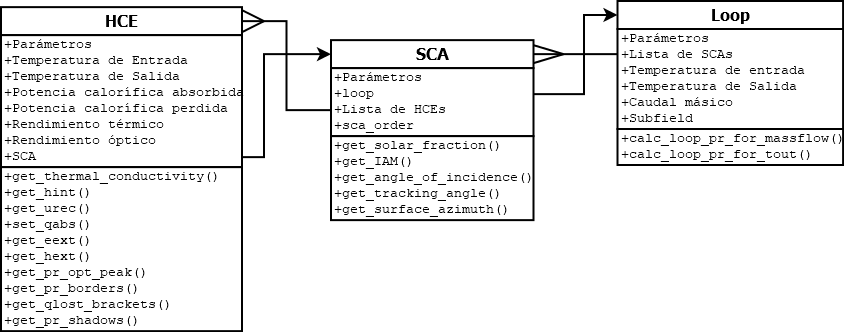
\includegraphics[width=0.9\linewidth]{images/clasescsenergy1.png}
\caption[Esquema relacional de las Clases HCE, SCA y Loop]{Esquema relacional de las Clases HCE, SCA y Loop. Se muestran los principales atributos y métodos de cada clase} 
\label{fig:clasescsenergy1}
\end{figure}

Un subcampo o sección es un conjunto de lazos conectados en paralelo, de tal forma que se espera que el caudal que circula por cada uno de sus lazos sea el mismo. El subcampo cuenta con válvulas de regulación de caudal a su entrada, por lo que constituye la unidad mínima de control de caudal en el campo solar. En algunas ocasiones cada lazo tiene capacidad de regulación de su caudal de forma constante. En ese caso se podría decir que cada lazo actúa como un subcampo con un único lazo, pero esto no es lo habitual.

Finalmente, el campo solar está formado por un conjunto de subcampos. El fluido caloportador frío entra en el campo solar y se distribuye por cada uno de los subcampos, donde se vuelve a distribuir equitativamente entre los lazos. En los lazos, el HTF se calienta y retorna a una tubería que lo conduce a la salida del subcampo, donde finalmente el HTF procedente de todos los subcampos se mezcla y se transporta, a lo largo de una tubería denominada colector caliente, hasta el punto de consumo. En la Fig.\ref{fig:clasescsenergy2} se esquematiza esta estructura de agregación de elementos. Cada Clase cuenta con métodos que permiten calcular los valores agregados de caudal, potencia y temperatura del fluido a partir de las aportaciones de cada uno de los subsistemas que engloba.

\begin{figure}[H]
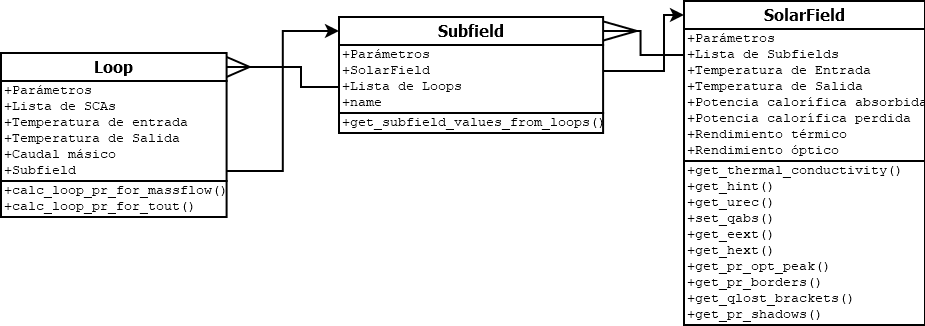
\includegraphics[width=0.9\linewidth]{images/clasescsenergy2.png}
\caption[Esquema relacional de las Clases SolarField, Subfield y Loop]{Esquema relacional de las Clases SolarField, Subfield y Loop. Se muestran los principales atributos y métodos de cada clase} 
\label{fig:clasescsenergy2}
\end{figure}


\subsection{Clases derivadas de Model: Clase \texttt{ModelBarbero4thGrade}, \\
\texttt{ModelBarbero1stGrade} y \texttt{ModelBarberoSimplied}}

Se emplean clases derivadas de la Clase \texttt{Model} para implementar los diferentes modelos empleados para calcular el rendimiento y para simular, por tanto, el funcionamiento de cada HCE. Es en cada una de estas clases donde se desarrolla el algoritmo que, a partir de los parámetros físicos que definen al HCE, las variables que definen el estado del HTF que circula por él y las condiciones de operación, resuelve las ecuaciones definidas en el modelo y nos permite conocer el rendimiento HCE.

\subsubsection{Clase \texttt{ModelBarbero4thOrder}}

La instancia de esta clase recibe como valores de entrada una referencia a una instancia de un HCE del cual va a calcular su rendimiento, una referencia a la instancia del HTF que se está empleando y valores de condiciones meteorológicas de radiación, temperatura y velocidad del viento. El HCE debe estar inicializado previamente con los valores de caudal másico, temperatura y presión de entrada y el flujo de calor absorbido \(\dot q_{abs}\).

El procedimiento de cálculo implementado en el método \emph{calc\_pr()} es el siguiente (los parámetros que se obtienen mediante métodos propios de las instancias del HCE y del HTF se explican en los apartados correspondiente más adelante): 
\begin{itemize}
\item
Estimación de la temperatura de pared exterior del tubo absorbedor \(T_{ro}\) según la ec\(\eqref{eq:tro}\) a partir del coeficiente de transmisión de calor al interior \(U_{rec}\) y del flujo de radiación absorbido por el tubo absorbedor, \(\dot q''_{abs}\), a partir de la instancia del HCE. Para el primer HCE del lazo se asume un rendimiento inicial \(\eta=1\) pero para los siguientes se emplea el rendimiento del HCE anterior, con lo cual se acelera un poco el proceso de convergencia por partirse de un valor previsiblemente más próximo.

\begin{equation}
    T_{ro} = T_f + \eta \cdot \frac{\dot q''_{abs}}{U_{rec}}
    \label{eq:tro}
\end{equation}

\item
  Cálculo del flujo de pérdidas \(\dot q''_{perd}\) mediante la   ec.\(\eqref{eq:qperd}\) incrementado con las pérdidas a través de los   soportes que sujetan el tubo absorbedor, \(\dot q_{perd,soportes}\).   Las pérdidas en los soportes se modelan mediante la   ec.\(\eqref{eq:qperdidassoportes}\) que se explica en el apartado   correspondiente de la clase HCE.
\item
  Cálculo de los parámetros de funcionamiento \(\dot q''_{crit}\),   \(U_{crit}\) y \(NTU\) para el HCE con la temperatura de pared   calculada previamente según las ecuaciones \(\eqref{eq:qcrit}\) y   \(\eqref{eq:ucrit}\) respectivamente.
\item
  Cálculo de los coeficientes \(f_1\), \(f_2\), \(f_3\) y \(f_4\)   mediante las ecuaciones \(\eqref{eq:f1}\) a \(\eqref{eq:f4}\) y   cálculo de \(f_0\) mediante la ec.\(\eqref{eq:f0}\).
\item
  Se resuelve la ec.\(\eqref{eq:rendimiento0}\) con de forma iterativa   mediante Newton-Raphson para calcular \(\eta_0\). Como valor inicial   se calcula \(\eta_0\) a partir de la   ec.\(\eqref{eq:rendimiento0aproximado}\) del Modelo de \(1^{er}\)  Orden.
\item
  Con el valor de \(\eta_0\) obtenido se calculan los valores de \(Z\),   \(g'(Z)\), \(g''(Z)\) y \(g'''(Z)\) dados por las ecuaciones   \(\eqref{eq:zeta}\) a \(\eqref{eq:g3primadezeta}\). 
\item
  Finalmente, se calcula el rendimiento \(\eta(x^*)\) según la   ec.\(\eqref{eq:modelocompleto}\), la temperatura de pared exterior   \(T_{ro}\) y se comparan con los valores iniciales. Si las diferencias   son superiores a cierto margen configurable se vuelve a realizar otra   iteración hasta conseguir la convergencia, pero previamente a cada iteración se re-calculan todos los pasos anteriores empleando la   temperatura de pared del tubo absorbedor calculada con el nuevo rendimiento. 
\end{itemize}

Al inicio del prcoeso iterativo se consdiera que, para el primer HCE del lazo, la temperatura del fluido \(T_f\) es igual a la temperatura de entrada al lazo (y al HCE, por tratarse del primero). Para los siguientes HCEs del lazo se parte de una temperatura del fluido igual a la temperatura de salida del HCE anterior pero incrementada con la mitad del salto de temperatura que experimentó dicho HCE.

Una vez finalizado el proceso iterativo, la instancia del HCE actualiza sus valores de rendimiento, temperatura y presión de salida del HTF, quedando totalmente definido su punto de funcionamiento. Las condiciones de temperatura y presión a la salida del HCE serán las de entrada del HCE siguiente.

Al calcular el rendimiento integral para todo la longitud del HCE estamos haciendo coincidir el tamaño de la malla de integración con la longitud física real del HCE. Se ha comprobado que la reducción de la malla no aumenta de forma apreciable la precisión de los cálculos y en cambio sí supone un coste computacional importante. Por el contrario, una forma de acelerar el proceso de simulación consiste en considerar artificialmente que la longitud del HCE es mayor que la real. Se trata de aumentar el tamaño de la malla de integración para reducir el número de cálculos. En este trabajo se seguirá, al igual que en \cite{barberofresnoDesarrolloModeloTeorico2018}, el criterio de no superar un tramo de HCE superior a 100 m propuesto en \cite{forristallHeatTransferAnalysis2003} para análisis unidimensional. 

\subsubsection{Clases \texttt{ModelBarbero1stOrder}  y \texttt{ModelBarberoSimplified}}

El proceso para el cálculo del rendimiento que realizan estas dos clases es similar al del Modelo de 4$^o$ Orden, salvo que ahora, el cálculo del rendimiento es explícito y no es necesario recurrir a la resolución de las ecuaciones por metodos numéricos, sino que se emplean directamente las ecuaciones   \(\eqref{eq:primerorden}\) y \(\eqref{eq:modelosimplificado}\) respectivamente. Una vez calculado el rendimiento, el algoritmo recalcula los valores hallados al inicio de la iteración y si la diferencia es mayor a los valores consignados, realiza una nueva iteración hasta alcanzar la convergencia deseada.


\subsection{Clase \texttt{HCE} para modelado del Heat Collector Element}
\label{heat-collector-element-hce}

De cara a modelar el funcionamiento del HCE como elemento responsable de calentar el HTF de forma compatible con el Modelo físico desarrollado, se define la Clase \texttt{HCE}, entre cuyos atributos se encuentran: temperatura de entrada del HTF, $T_{in}$ (internamente el programa trabaja con K como unidades de temperatura, aunque la entrada y salida de datos se realiza con $^\circ C$); potencia calorífica absorbida a lo largo de todo el HCE, $\dot q_{abs}$ (W); potencia calorífica perdida a lo largo del HCE, $\dot q_{perd}$ (W); rendimiento óptico del conjunto HCE+SCA, $\eta_{opt}$; rendimiento térmico, $\eta$ y temperatura de salida, $T_{out}$, (K). 

El caudal másico de HTF que circula por el HCE, $ \dot m $ (kg/s) se obtiene mediante una referencia al SCA y, seguidamente, otra referencia al Loop que contienen al HCE. 

Con estos parámetros el comportamiento del HCE queda totalmente caracterizado en el sistema desde el punto de vista del proceso de generación. Estos atributos (pueden entenderse como variables) están relacionados entre sí según las reglas que aplique cada modelo. La temperatura de salida del HTF, $T_{out}$, aparece implícita en la ec.\ref{eq:deltaH}:

\begin{equation}
    \dot H =  \dot m  \int^{T_{out}}_{T_{in}}c_p(T) dT 
    \label{eq:deltaH}
\end{equation}

donde \(\dot H\) representa una tasa temporal de incremento de entalpía, pues hemos considerado que se trata de un fluido incompresible y también se ha despreciado la participación de energía cinética, por lo que la potencia térmica se invierte en incrementar la entalpía del sistema. Previamente se debe calcular \(\dot H\) según la ec.\(\eqref{eq:delta_hvalor}\):

\begin{equation}
   \dot H =  \dot q''_{abs} \cdot \eta \cdot \pi \cdot D_{ro} \cdot L \cdot \gamma_L \cdot \gamma_g
    \label{eq:delta_hvalor}
\end{equation}

La ec.\(\eqref{eq:deltaH}\) puede resolverse por métodos numéricos si el calor específico \(Cp\) del fluido se ha obtenido a partir de un polinomio. En el caso de que se disponga de una función que proporcione la temperatura del fluido en función de la entalpía \(T(h)\), como ocurre si se usa \(CoolProp\), se puede calcular su valor directamente a través de las funciones que ofrece esta librería como \(T_{out} = T(h_{out})\).

En la ec.\ref{eq:delta_hvalor} se introducen el \textit{factor de longitud efectiva}, \(\gamma_L\) y \textit{factor de interceptación geométrico}, \(\gamma_g\) para tener en cuenta la reducción de la longitud \textit{activa} del HCE debido a los fuelles en los extremos del HCE y al sombreado del escudo térmico en las uniones de HCEs. Un valor típico para ambos factores está comprendido entre 0,96 y 0,97 \cite{zarzaApuntesMasterConsultor2006}. En el caso de que el calor absorbido sea nulo, la temperatura de salida será inferior a la de entrada y el valor \(\dot H < 0\). En este caso, no existe reducción de la longitud efectiva del absorbedor y la energía perdida se calcula según la ec.\(\eqref{eq:delta_hvalornegativo}\) pues a lo largo de toda la superficie del HCE se experimentan pérdidas energéticas:

\begin{equation}
   \dot H =  \dot q''_{perd} \cdot \pi \cdot D_{ro} \cdot L
    \label{eq:delta_hvalornegativo}
\end{equation}

\subsubsection{Cálculo del flujo de calor absorbido, $\dot q''_{abs}$}

La radiación que alcanza al fluido caloportador puede obtenerse mediante la ec.\ref{eq:qabs}:
\begin{equation}
\notag \dot q''_{abs}= \eta_{opt}(\theta) \cdot Cg \cdot DNI \cdot \eta_{sombras} \cdot \eta_{bordes}  \tag{\ref{eq:qabs}}
\end{equation}

donde \(DNI\) es la radiación normal directa cuyo valor se lee para cada  fecha de cálculo de la simulación. \(Cg\) es el factor de concentración geométrica, definido genéricamente   para sistemas de concentración como el cociente entre el área de  apertura del concentrador, \(A_c\) y la superficie del receptor,   \(A_{ext}\). Hemos considerado como efectiva toda el área del receptor, no solo aquella donde se concentra la radiación, ya que supondremos que el flujo se reparte uniformemente por toda la superficie de tubo absorbedor. De esta manera, el área de apertura de un concentrador de longitud $L$, con una longitud de apertura de su superficie parabólica $A_p$, viene dado por la ecuación:

\begin{equation}
   A_c = A_p \cdot L
    \label{eq:aperturaconcentrador}
\end{equation}

y la superficie del receptor, de igual longitud $L$ y diámetro exterior del tubo absorbedor $D_{ro}$, es:

\begin{equation}
   A_{ext} = \pi \cdot D_{ro} \cdot L
    \label{eq:superficiereceptor}
\end{equation}

De esta manera,  el factor de concentración geométrica para un colector cilindroparabólico se calcula según la ec.\(\eqref{eq:cg}\):

\begin{equation}
   Cg = \frac{A_p}{\pi \cdot D_{ro}}
    \label{eq:cg}
\end{equation}


El rendimiento óptico \(\eta_{opt}(\theta)\)  depende del   ángulo de incidencia \(\theta\) y se obtiene a partir del rendimiento  óptico pico, \(\eta_{opt,peak}\) y del modificador del ángulo de   incidencia, \(IAM\) según la ec.\(\eqref{eq:rendimientooptico}\):


\begin{equation}
   \eta_{opt}(\theta) = \eta_{opt,peak} \cdot IAM \cdot cos(\theta)
    \label{eq:rendimientooptico}
\end{equation}

Esta ecuación incluye también el coseno del ángulo de incidencia pues consideraremos que, en general, no está incluido este término dentro de IAM. En caso de que la expresión del $IAM$ ofrecida por el fabricante ya incluyese este efecto, debería eliminarse de la ecuación (\ref{eq:rendimientooptico}). 
Para calcular \(\eta_{opt,peak}\) empleamos la expresión dada en la ec.\(\eqref{eq:rendimientoopticopico}\). 

\begin{equation}
   \eta_{opt,peak} = \alpha \cdot \tau \cdot \rho \cdot \gamma
    \label{eq:rendimientoopticopico}
\end{equation}

La ecuación para \(IAM\) se ofrece en la sección correspondiente al modelado del SCA ya que es una propiedad más propia del sistema de concentración y seguimiento. La instancia del HCE hace una llamada al método \emph{get\_IAM} de su SCA asociado, aquel en el que está montado, para recibir su valor. Igualmente, en la ec.\(\eqref{eq:rendimientoopticopico}\) los parámetros \(\rho\) (reflectividad del concentrador) y \(\gamma\) (fracción solar), son parámetros del SCA y deben obtenerse de la instancia de SCA asociada al HCE. \(\alpha\) es la absortividad del receptor y \(\tau\) es la transmisividad del vidrio envolvente del tubo absorbedor. En ambos casos se trata de parámetros configurables que se introducen con el resto de características del HCE en el archivo de configuración de la simulación.

El factor \(\eta_{bordes}\) contabiliza las pérdidas debidas a que en una   pequeña porción del tubo absorbedor del SCA no se produce   concentración debido al ángulo de incidencia. Un tramo del tubo   absorbedor, que puede implicar desde solo un tramo del primer HCE  hasta a varios HCEs, tendrá un flujo de radiación nulo, o muy bajo. El   tramo de tubo absorbedor que queda sin concentración (\(L_{bordes}\)   se calcula mediante la ec.\(\eqref{eq:bordes}\) a partir de la   distancia focal, \(f_l\) y de ángulo de incidencia \(\theta\):

\begin{equation}
   L_{bordes} = \frac {f_l}{tan(\theta)}
    \label{eq:bordes}
\end{equation}

A partir de este valor el código calcula que fracción del HCE o cuantos HCEs quedan inutilizados y les asigna un rendimiento nulo.

En el caso del factor \(\eta_{sombras}\), se trata de un valor que se calcula en base a la porción del concentrador que se encuentra afectado por sombras debido a que la distancia de separación entre lazos está acotada. En disposiciones de lazos habituales con eje seguimiento Norte-Sur estas sombras solo aparecen a primera y última hora del día. Su cálculo exacto según se describe en \cite{sharmaShadingAvailableEnergy2013} requeriría conocer completamente la disposición de cada lazo en cada instante, pero una aproximación suficiente se puede conseguir según la ec.(\eqref{eq:sombras}) tal y como hace SAM, \cite{gilmanSolarAdvisorModel2008}:

\begin{equation}
   \eta_{sombras} =  \frac {cos(\beta) \cdot D_L}{A_c}
    \label{eq:sombras}
\end{equation}

donde $\beta$ es el ángulo de seguimiento, $D_L$ es la distancia de separación entre lazos y $A_c$ es la apertura del concentrador.

\subsubsection{Pérdidas en el tubo absorbedor, $\dot q''_{perd}$}

Las pérdidas se modelan según la ec.(\ref{eq:qperd}), que repetimos a continuación:

\begin{equation}
\notag  \dot q''_{perd}(x)= \sigma \cdot \varepsilon_{ext} \cdot (T_{ro}^{4}(x)-T_{ext}^{4}) + h_{ext} \cdot (T_{ro}(x)-T_{ext}) \tag{\ref{eq:qperd}}
\end{equation}

donde   \(\varepsilon_{ext}\) es la \textit{emisividad equivalente de la superficie  exterior} del receptor. Depende de la temperatura de pared exterior del tubo y se emplea la ec.\(\eqref{eq:eext}\) para calcularla:

\begin{equation}
   \varepsilon_{ext} =  A_0 + A_1 \cdot  (T_{ro} - 273.15)
    \label{eq:eext}
\end{equation}

Se corrige ligeramente su valor en función de la velocidad del viento, incrementando su valor un 1\% con un viento de 4 m/s y un 2\% para viento de 7 m/s. Los coeficientes \(A_0\) y \(A_1\) son los que se ofrecen en \cite{barberofresnoDesarrolloModeloTeorico2018}.

Por otro lado,  \(h_{ext}\), es el \textit{coeficiente de transferencia de calor convectivo  equivalente al exterior}. Su valor puede considerarse nulo para el caso  de un HCE con vacío en su espacio anular. Nuevamente, en \cite{barberofresnoDesarrolloModeloTeorico2018} se ofrecen las ecuaciones para diferentes combinaciones de   recubrimiento, Black-Chrome o Cermet y conservación o no del vacío,   obtenidas mediante simulación CFD (Computational Fluid Dynamics) por su autor para un modelo unidimensional del HCE. A falta de datos para los modelos concretos empleados en este trabajo, en todas nuestras simulaciones consideraremos que su valor es nulo (equivalente a un caso de velocidad de viento nula), lo cual es aceptable en etapas de prediseño de plantas o durante análisis paramétrico.

Se incluye en el modelado el cálculo de las pérdidas a través de los soportes que sujetan al HCE, \(\dot q_{perd,soportes}\). Su peso relativo en el total de pérdidas del campo no es muy elevado, por lo que, a falta de más datos, se hace uso de la ec.\(\eqref{eq:qperdidassoportes}\)  propuesta en \cite{forristallHeatTransferAnalysis2003}:

\begin{equation}
   \dot q_{perd,soportes} =  n \cdot \frac{\sqrt{P_b \cdot k_b \cdot A_{cs,b} \cdot \bar h_b} \cdot (T_{base} - T_{ext})}{L}
    \label{eq:qperdidassoportes}
\end{equation}

donde \(P_b\) es el perímetro de la sección del soporte ($0,2032\,m$), \(A_{cs,b}\) es la sección transversal de la unión entre el brazo y el tubo absorbedor ($1,613\cdot 10^{-4}\,  m^2$), \(K_b\) es la conductividad térmica del acero empleado en el brazo ($48,0\,W/(m \cdot K)$), \(\bar h_b\) es el coeficiente de transmisión de calor por convección medio hacia el exterior ($20\, W/(m^2 \cdot K)$), \(T_{base}\) es la temperatura de la zona de conexión entre los brazos y el tubo absorbedor, \(L\) es la longitud del colector y \(n\) es el número de soportes por colector.

\subsubsection{Otros atributos y métodos de la Clase \texttt{HCE}}

Ya hemos visto, al hablar de la Clases para los modelos, cómo un objeto (instancia) de la clase HCE puede ser procesada por otra instancia de la clase del modelo para simular su comportamiento. Es necesario que la instancia del HCE pase los siguientes parámetros al modelo:

\begin{itemize}
\item
  \(k_{rec}\), conductividad térmica de la pared del receptor. Se ha  empleado la ec.\(\eqref{eq:krec}\) válida para el acero inoxidable
  321H:

\begin{equation}
    k_{rec} = 0,0153 \cdot (T - 273,15) + 14,77
    \label{eq:krec}
\end{equation}
\end{itemize}

\begin{itemize}
\item
  \(h_{int}\), coeficiente de transferencia de calor convectivo hacia el   interior. Para el cálculo se emplea la ec.\(\eqref{eq:hint}\) donde   \(Nu_{G}\) es el número de Nusselt obtenido mediante la correlación de   Gnielinski dada en la ec.\(\eqref{eq:nug}\), \(D_{ri}\) es el diámetro   interior del tubo absorbedor y \(k_f\) es la conductividad térmica a   la temperatura del fluido: 
\begin{equation}
    h_{int} = \frac{Nu_{G}\cdot k_f }{D_{ri}}
    \label{eq:hint}
\end{equation}

\begin{equation}
    Nu_{G} = \frac{ \left( \frac{C_f}{2} \right)\cdot\left( Re_{D_{ri}} - 1000 \right)\cdot Pr_f }{1 + 12,7 \cdot \left(\frac{C_f}{2} \right)^{\frac{1}{2}}\cdot \left(Pr^{\frac{2}{3}}_f -1 \right)} \cdot \left( \frac{Pr_f}{Pr_{ri}} \right)^{0,11}
    \label{eq:nug}
\end{equation}

\item
  \(U_{rec}\), coeficiente de transmisión de calor al interior. Viene   dado por la ec.\(\eqref{eq:urec}\) comentada previamente. 
\end{itemize}

La Clase \texttt{HCE} también nos proporciona algunos métodos necesarios para el trabajo de procesamiento de la información, asignación y recuperación de valores de los atributos. Otro aspecto importante es que cada instancia de la clase \texttt{HCE} tiene un
atributo de tipo \emph{diccionario} denominado \texttt{parameters}  en el que, a modo de lista de pares clave-valor, va a recibir aquellos parámetros que posteriormente serán empleados por el Modelo. Los diferentes autores que han elaborado modelos para los HCE no siempre utilizan los mismos parámetros ni idénticos identificadores. Al emplear un diccionario se facilita la tarea de implementación de nuevos Modelos, sin que sea necesario cambiar los atributos de la clase en cada ocasión. Entre los parámetros que se
pasan al HCE durante la creación de su instancia están su absortividad solar \(\alpha_{solar}\), la transmisividad del vidrio \(\tau\) y su reflectividad \(\rho\).

En el caso de la planta simulada se ha utilizado un HCE fabricado por Solel cuyos parámetros se guardan en una librería en formato JSON. Parte de los datos de cada HCE de la librería se han extraído de los archivos de configuración de SAM (System Advisor Model), el software de referencia para la simulación de plantas de energías renovables. No obstante, el modelo no hace uso de todos ellos y, en cambio, se precisa de algún dato más para realizar la simulación. Estos parámetros son
almacenados en el diccionario \emph{parameters}. El programa desarrollado permitiría, en principio, modelar cada HCE con unos parámetros diferentes, es decir, que cada HCE se comportase de forma diferente al resto. Esta funcionalidad puede ser interesante para el estudio de comportamiento del campo solar cuando se dispone de estadísticas adecuadas sobre cómo evoluciona en el tiempo y se distribuye en el campo solar cada parámetro, lo cual hace que no todos los lazos se comporten de igual manera. El inconveniente es que el tiempo de cálculo aumenta notablemente al tener que simularse cada lazo independientemente. 


\subsection{Clase \texttt{SCA}, para el modelado del Solar Collector Assembly}
\label{solar-collector-assembly-sca}

Un SCA es una estructura compuesta por una serie de reflectores que concentran la radiación solar sobre los HCE. Desde el punto de vista operativo, un SCA cuenta con capacidad de movimiento independiente respecto al resto de SCAs de la planta, por lo que es la unidad mínima de control de enfoque o desenfoque de la radiación solar en el campo solar. La clase SCA nos permite modelar cada SCA teniendo en cuenta las propiedades de los reflectores (reflectividad, suciedad de los espejos, precisión del movimiento de seguimiento solar, etc.)

En plantas CCP dedicadas a maximizar la generación anual de energía eléctrica, el sistema de seguimiento tiene su eje de rotación alineado en la dirección Norte-Sur con el fin de hacer un seguimiento Este-Oeste de la trayectoria solar a lo largo del día. No obstante, una configuración con eje Este-Oeste también puede ser interesante en algunos casos y el modelo también permite esta configuración.

Dentro del campo solar, cada HCE debe pertenecer a un SCA. El primer HCE del SCA recibe el fluido caloportador procedente de otro SCA o de las tuberías colectoras de HTF frio. El último HCE del SCA entrega el HTF más caliente al siguiente SCA o a las tuberías colectoras de HTF caliente a la salida del lazo.

El SCA cuenta con un método para el cálculo del modificador por ángulo de incidencia. Hemos considerado que el SCA mantendrá en todo momento un ángulo de seguimiento \(\beta\) óptimo con el fin de minimizar el ángulo de incidencia. En este caso, el \(IAM\) se calcula según la expresión dada por la ec.\(\eqref{eq:iam}\)

\begin{equation}
   IAM = F_0 + F_1 \cdot \frac{\theta}{cos(\theta)} + F_2 \cdot \frac{\theta^2}{cos(\theta)},\,\, \forall  \,
 \theta \in (0^o, 80^o)
    \label{eq:iam}
\end{equation}

Algunos fabricantes incluyen un factor \(cos(\theta)\) en la expresión del \(IAM\), por lo que no deberá incluirse entonces en la ecuación del rendimiento total del HCE. En nuestro caso, para el UVAC 3 de Solel empleado en la simulación, no es así.

Otro valor que debe ofrecernos la clase que modela al SCA es la \textit{fracción solar} o \textit{factor de interceptación}, que permite estimar la tasa entre la radiación solar que alcanza al reflector y la que posteriormente indice realmente sobre el tubo absorbedor. Su valor se obtiene según la ec.\(\eqref{eq:fraccionsolar}\) como producto de una serie de factores: 

\begin{equation}
   \gamma = \eta_{geométrico} \cdot \eta_{seguidor} \cdot \eta_{suciedad} \cdot \eta_{disponibilidad}
    \label{eq:fraccionsolar}
\end{equation}

El factor geométrico \(\eta_{geométrico}\) depende de las imperfecciones geométricas de conjunto reflector-absorbedor como pequeñas desviaciones en la curvatura de los espejos o la deformación de la estructura. El factor de precisión del seguidor \(\eta_{seguidor}\) permite considerar los errores de seguimiento del mecanismo de movimiento del reflector. El factor de suciedad \(\eta_{suciedad}\) se refiere a la pérdida de reflectividad debida a acumulación de polvo en los espejos. Se ha considerado que esta acumulación de polvo afecta también a la transmisividad de la cubierta de vidrio del HCE, por lo que este factor se computa dos veces. Finalmente, el factor de disponibilidad \(\eta_{disponibilidad}\) considera las pérdidas que ocasionalmente se puedan producir por averías del sistema de concentración.

El SCA, como sistema responsable del seguimiento solar, también cuenta con un método para ofrecernos información sobre el ángulo de incidencia \(\beta\) en el plano de apertura del reflector. Las expresiones generales pueden encontrarse en \cite{duffieSolarEngineeringThermal2006} pero, en nuestro caso, hemos recurrido a la librería \emph{pvlib-python}  \cite{holmgrenPvlibPythonPython2018}, desarrollada en \emph{Sandia National Laboratories} con el objetivo de impulsar el desarrollo de herramientas de código abierto para la simulación de sistemas fotovoltaicos. Concretamente, nos valemos de este código para obtener los valores del ángulo de incidencia y la posición solar para cada fecha del año según las coordenadas geográficas del lugar donde se realiza la simulación.

\subsection{Clase \texttt{Loop}}
\label{loop}

Un Loop o lazo es un conjunto de SCAs conectados en serie de tal forma que el HTF que entra frío al lazo experimenta un salto térmico cuando transita por él. El sistema de control ajusta el estado de enfoque o desenfoque de cada SCA en el lazo con el fin de conseguir que la temperatura de salida sea la de consigna. Por motivos de económicos, el caudal de HTF no suele ser regulable a nivel de lazo, pues obligaría a instalar una válvula de control en cada uno de ellos, por lo que todos los lazos de un mismo subcampo suelen tener un caudal muy parecido. Se ha desarrollado también una Clase Subfield para dar cuenta del conjunto de lazos que pertenecen a un mismo subcampo y, por tanto, pueden variar su caudal de forma independiente de los lazos de otro subcampo. En un campo solar suele haber haber varios subcampos que pueden regular su caudal independientemente. Los casos más extremos serían el de un campo solar con un único subcampo, en el que todos los lazos pertenecen al mismo subcampo y en el otro extremo, un campo solar con tantos subcampos como lazos tiene, de tal forma que cada lazo es el único en su subcampo y por tanto cada lazo puede regular su caudal independientemente. 

Cada lazo del campo solar es modelado mediante una instancia de la clase Loop. Cada instancia mantiene referencias al subcampo al que pertenece y a los SCA que contiene. Atributos importantes de estas instancias serán el caudal de HTF en el lazo, las temperaturas de entrada y salida del HTF y el rendimiento completo del lazo. 

El código permite trabajar de dos formas: 

\begin{itemize}
\item
Método \texttt{calc\_loop\_pr\_for\_tout}, que calcula el caudal requerido con el que conseguir una temperatura de HTF determinada.
\item
Método \texttt{calc\_loop\_pr\_for\_massflow}, que  mantiene fijo el caudal de HTF que se le indica y calcula qué temperatura de salida alcanzará el HTF. 
\end{itemize}

En caso de que esta temperatura de salida supere el máximo permitido (un valor configurable) se producirá un desenfoque en el SCA en que se alcance esta temperatura y el HTF dejará de calentarse. En este caso se suele decir que se produce un vertido de energía o desaprovechamiento de la radiación existente. El código permite contabilizar esta energía desaprovechada por cada lazo durante estas situaciones.

La Clase \texttt{BaseLoop} hereda de la Clase \texttt{Loop} sus principales métodos y atributos pero supone una pequeña variación de una instancia o lazo definido por Loop ya que se trata de un lazo  "típico'' o "promedio'', que presenta una configuración constructiva idéntica a la del resto de lazos de la planta pero no pertenece a ningún subcampo solar. Este lazo especial o prototipo se empleará cuando queramos realizar un estudio paramétrico del comportamiento del lazo, no de la planta, y también para realizar una simulación mucho más rápida cuando asumamos la hipótesis de que todos los lazos de la planta se comportan de igual manera. Esta aproximación es la que se hace en aplicaciones como SAM, donde no se simulan todos los lazos para modelar el campo solar, sino que se simula solo un lazo y el resultado se obtiene multiplicando el caudal de salida de este lazo por el número de lazos que forman la planta. 

\subsection{Clase \texttt{Subfield}, modelado del subcampo}
\label{subfield}

Un subcampo es un conjunto de lazos en los que se considera que el HTF se repartirá equitativamente. Cada subcampo dispone de una válvula de control de caudal a su entrada y representa el mayor grado de control de caudal de HTF que se puede alcanzar en el campo solar. Un campo solar suele contar con varios subcampos y cada uno de ellos, a su vez, cuenta con varios lazos.  

La Clase \texttt{Subfield} mantiene referencias a lo lazos que lo constituyen, es decir, a cada una de las instancias que representan un lazo. También mantiene referencia al campo solar al que pertenece y cuenta con métodos para calcular cual será la temperatura de salida del HTF del subcampo solar una vez que el caudal de salida de cada lazo se haya mezclado con el del resto de lazos. Nótese que aunque se supone que todos los lazos del subcampo tienen el mismo caudal másico la temperatura de salida de cada uno de ellos puede ser diferente y, por tanto, la energía aportada por cada lazo también lo será. 

\subsection{Clase \texttt{Solarfield}, modelado del campo solar}
\label{solarfield}

El campo solar alberga el conjunto de subcampos y, por tanto, todos los lazos de la instalación. Se trata del objeto que en última instancia queremos modelar con el fin de conocer cómo sera el comportamiento de la planta solar y su rendimiento anual. A la hora de definir el campo solar para el modelo es necesario conocer cuántos subcampos contiene, cuántos lazos hay en cada subcampo, qué configuración tiene cada lazo (número de SCAs en cada lazo y número de HCEs en cada SCA). También es importante conocer la distancia entre lazos con el fin de estimar el sombreado que se produce a primera y última hora del día. 

El Clase \texttt{Solarfield} también recibe una serie de valores nominales para los que se ha realizado un diseño óptimo del sistema, como las temperaturas y presiones de entrada y salida del HTF, las temperaturas máximas y mínmas tolerables por razones de seguridad, el caudal nominal (normalmente se suele dar este caudal por lazo y el caudal del campo solar será la suma de todos ellos), el caudal mínimo (existe cierta limitación tanto por la velocidad mínima de las bombas como por otras
cuestiones operativas que desaconsejan que el HTF circule por debajo de este límite).

Cuando se crea una instancia de la Clase \texttt{Solarfield}, ésta recibe los datos de configuración que se han pasado para la simulación y lanza el proceso de construcción que genera, en base a esa configuración, los diferentes subcampos, lazos, SCAs y HCEs que forman el campo solar.

\subsection{Clase \texttt{Fluid} y sus clases hijas, \texttt{FluidCoolProp} y \texttt{FluidTabular}}
\label{subclases-fluid}

Para modelar el HTF (Heat Transfer Fluid) se ha creado la Clase Fluid. Las propiedades del HTF pueden obtenerse mediante funciones polinómicas con coeficientes constantes calculados experimentalmente o desde librerías preexistentes como \textit{CoolProp}. Por ese motivo, según se opte por un método u otro, se han creado las subclases \texttt{FluidCoolProp} y \texttt{FluidTabular}. No obstante, se ha comprobado que el número de fluidos existentes en la librería FluidCoolProp que suelen emplearse como HTF no es muy grande, limitándose a \emph{Therminol VP-1} y \emph{Syltherm 800}. No se encuentra en esta librería el aceite \emph{Dowtherm-A}, que es el que se emplea en la planta cuyos datos se han empleado para el desarrollo de esta herramienta. Pero el mayor inconveniente reside en que \emph{CoolProp} devuelve valores solo dentro del rango de temperaturas de uso válidas según el fabricante. 

Este rango es demasiado estricto y se producen problemas debido a la devolución de valores no numéricos, especialmente cuando se está calculando la temperatura teórica de salida del HTF en condiciones de sobrecalentamiento. Por este motivo, se ha hecho uso mayoritariamente de la clase \texttt{FluidTabular}, con funciones polinómicas con coeficientes calculados a partir de los datos ofrecidos por los fabricantes.  La clase \texttt{Fluid} y sus clases hijas ofrecen métodos para calcular la densidad, viscosidad cinemática, número de Reynolds, calor específico, conductividad térmica y entalpía en función de la temperatura y la presión. También ofrecen un método para calcular la temperatura del fluido en función de la entalpía y la presión, considerando entalpía cero para líquido saturado según ASHRAE a una temperatura de 285,856 K.

Para el modelado sería necesario conocer la dependencia de los parámetros citados en función de la temperatura y la presión, pero se ha comprobado que la variación de estos parámetros con la presión es despreciable cuando se trabaja en condiciones de líquido saturado. Ya que en una planta termosolar se debe trabajar siempre con esta premisa, estando los circuitos de HTF siempre bien presurizados, expresaremos dichos parámetros  a partir de un polinomio de mayor o menor grado, en función exclusivamente de la temperatura. También se ha obtenido una curva para calcular la temperatura del líquido saturado en función de su entalpía.

\begin{itemize}
\item
  $\rho(T)$: Densidad, $(kg/m^3)$
\item
  $\mu(T)$: Viscosidad dinámica, $(Pa \cdot m)$
\item
  $k_T(T)$: Conductividad térmica, $(W/m \cdot K)$
\item
  $c_p(T)$: Calor específico a presión constante, $(J/kg\cdot K)$
\item
$h(T)$: Entalpía específica, $(J/kg)$, considerando h=0 a $T_{ref}= 285,86 K$
\item
$T(H)$: Temperatura en función de la entalpía, (K)
\end{itemize}

La fórmula general para cada uno de estos parámetros es del tipo de la ec.\(\eqref{eq:polinomiohtf}\):

\begin{equation}
   parámetro(T) = a_0 + a_1 \cdot T + a_2 \cdot T^2 + a_3 \cdot T^3 + a_4 \cdot T^4 + a_5 \cdot T^5 + a_6 \cdot T^6 +  a_7 \cdot T^7 + a_8 \cdot T^8   
    \label{eq:polinomiohtf}
\end{equation}

No todos los parámetros requieren un polinomio de grado tan alto y los coeficientes que acompañan a los términos de mayor grado son nulos, pero se ha empleado esta estructura por homogeneizar el proceso de carga de datos.

Para el caso del \emph{Dowtherm-A} se han obtenido los coeficientes de los polinomios que caracterizan cada parámetro a partir de \cite{richardl.mooreImplementationDOWTHERMProperties2010} y se han contrastado las curvas con los datos ofrecidos en \cite{machadoProductTechnicalData}. En el caso de la viscosidad cinemática se ha detectado que el polinomio de 8º grado que se obtiene con los coeficientes de la primera referencia presenta una gran desviación y crecimiento asintótico para temperaturas ligeramente superiores a la máxima de operación del fluido. Con el fin de poder flexibilizar el proceso de cálculo y que no se produzcan desbordamientos se ha ajustado un nuevo polinomio tras extender los datos de la viscosidad dinámica hasta unos 450 °C aproximadamente según la tendencia observada en el último tramo de la curva \(\mu(T)\). De esta forma se obtiene un nuevo polinomio, con mejor comportamiento en este rango extendido.

En las figuras \ref{f:parametros_dowa} puede verse el comportamiento estos parámetros en función de la temperatura para el caso del \emph{Dowtherm-A}.

\begin{figure}
  \subfloat[Densidad]{
   \label{f:densidad}
    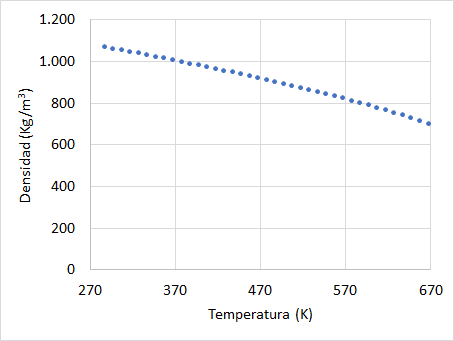
\includegraphics[width=0.5\textwidth]{images/densidad_dowa.png}}
  \subfloat[Viscosidad dinámica]{
   \label{f:viscosidad}
    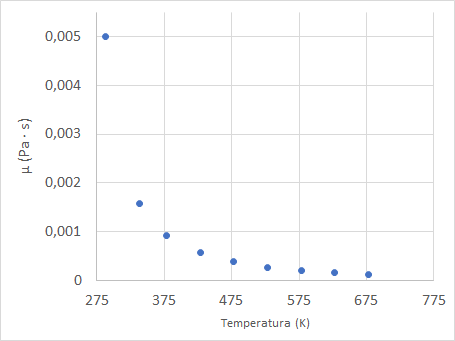
\includegraphics[width=0.5\textwidth]{images/viscosidaddinamica_dowa.png}}
  \\
   \subfloat[Conductividad térmica]{
   \label{f:kt}
    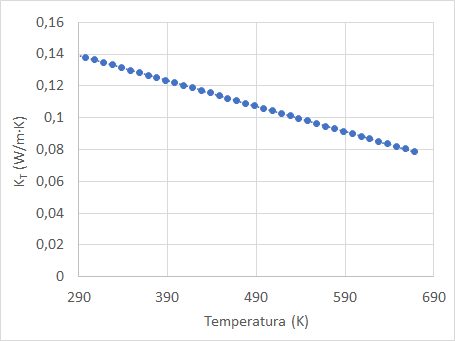
\includegraphics[width=0.5\textwidth]{images/conductividad_dowa.png}}
   \subfloat[Calor específico a presión constante]{
   \label{f:cp}
    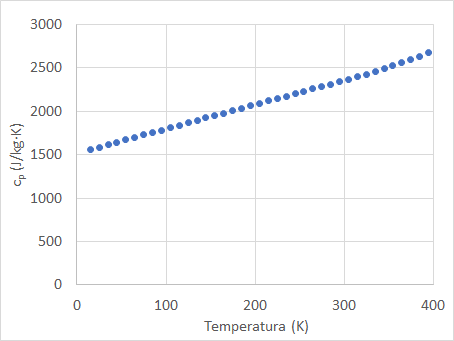
\includegraphics[width=0.5\textwidth]{images/calorespecifico_dowa.png}}
  \\
   \subfloat[Temperatura]{
   \label{f:temperatura}
    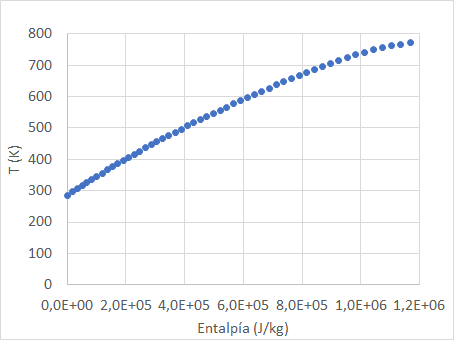
\includegraphics[width=0.5\textwidth]{images/temperatura_dowa.png}}
   \subfloat[Entalpía]{
   \label{f:entalpia}
    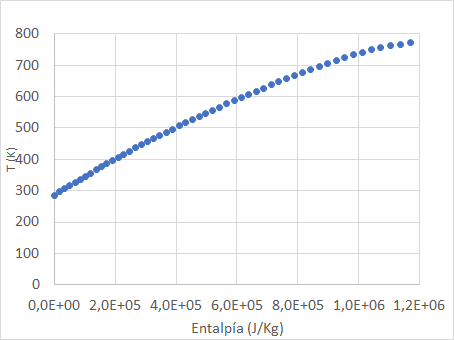
\includegraphics[width=0.5\textwidth]{images/entalpia_dowa.png}}
 \caption[Parámetros fisicos del \emph{Dowtherm-A} en estado de líquido saturado]{Parámetros fisicos del \emph{Dowtherm-A} en estado de líquido saturado. Algunos puntos se han extrapolado más alla de la temperatura máxima de trabajo con el fin de evitar errores durante los procesos de convergencia.}
\label{f:parametros_dowa}
\end{figure}

Los coeficientes de los polinomios de ajuste para \emph{Dowtherm-A} se muestran en la tabla \ref{tab:coeficientes_dowa}:

\begin{table}[H]
\centering
\caption[Coeficientes polinómicos para el fluido caloportador \emph{Dowtherm-A}]{Coeficientes polinómicos para el fluido caloportador \emph{Dowtherm-A}}
\label{tab:coeficientes_dowa}
\resizebox{0.9\textwidth}{!}{%
\begin{tabular}{lcccccc}
Parámetro	& $C_p(T) $	& $\mu(T)$	& $\rho(T)$  & $K_T$      	&  H(T)		& T(H)        \\ \hline
$a_0$ 		& -2,36E+03	& 1,58E+00  & 1,49E+03  & 1,86E-01  	& -6,51E+05	& 2,85E+02 	\\
$a_1$		& 3,95E+01  & -2,34E-02 	& -3,33E+00 & -1,60E-04 	& 4,12E+03  & 6,21E-04  	\\
$a_2$ 		& -1,70E-01 	& 1,50E-04  	& 1,25E-02  	& 5,91E-12  	& -1,24E+01 & -1,82E-10 	\\
$a_3$ 		& 3,90E-04  	& -5,49E-07 	& -2,97E-05 	& 0,00E+00  & 2,77E-02  	& -1,42E-16 	\\
$a_4$ 		& -4,42E-07 	& 1,24E-09  	& 3,44E-08  	& 0,00E+00  & -2,78E-05 	& 3,32E-22  	\\
$a_5$ 		& 1,98E-10  	& -1,78E-12 	& -1,62E-11 	& 0,00E+00  & 1,11E-08  	& -1,75E-28 	\\
$a_6$		& 0,00E+00  & 1,58E-15  	& 0,00E+00  & 0,00E+00  & 0,00E+00 	& 0,00E+00  \\
$a_7$ 		& 0,00E+00  & -7,94E-19 	& 0,00E+00  & 0,00E+00  & 0,00E+00 	& 0,00E+00  \\
$a_8$ 		& 0,00E+00  & 1,73E-22  	& 0,00E+00  & 0,00E+00  & 0,00E+00 	& 0,00E+00 
\end{tabular}%
}
\end{table}

El mismo procedimiento se ha empleado para obtener los polinomios característicos del fluido \emph{Therminol VP-1}, aunque en este caso los polinomios se han ajustado a partir de una lista de valores sacada de la librería \emph{CoolProp}. Pese a que el programa de simulación permite que durante el tiempo de ejecución se obtengan los parámetros citados a través de esta librería, existe una limitación debido al rígido margen de temperaturas con el que esta librería trabaja para cada fluido y esto
provoca que, para valores de temperatura ligeramente superiores al rango de operación ofrecido por fabricante, no se devuelva ningún valor. Esto resulta en problemas en tiempo de ejecución si algún lazo alcanza una temperatura superior a los 397°C (398°C en el caso de Syltherm 800). Aunque superar esta temperatura no es recomendable, es algo que puntualmente ocurre durante la operación de la planta. Además, una forma calcular la energía desaprovechada por desenfoque sería a partir de la temperatura que hubiera alcanzado el lazo de no haberse producido el desenfoque y calculando posteriormente su entalpía. Esta aproximación, que sería imposible en la vida real debido a la degradación del HTF e incluso al daño del propio sistema por las sobrepresiones que se producirían, facilita el cálculo de la energía desaprovechada en cada  momento. Se ha supuesto que las curvas de los parámetros se mantienen bien ajustadas siempre y cuando la sobretemperatura alcanzada no sea excesiva (en las simulaciones realizadas no se ha superado más del 10\% de la temperatura máxima de operación recomendada por el fabricante). Por estos motivos, para este trabajo se han empleado siempre los valores de los parámetros obtenidos a partir de los polinomios y no de \emph{CoolProp}.

Para el caso del \emph{Therminol VP-1} los coeficientes calculados son los que se muestran en la tabla \ref{tab:coeficientes_vp1}:

\begin{table}[H]
\centering
\caption{Coeficientes polinómicos para el fluido caloportador \emph{Therminol VP-1}}
\label{tab:coeficientes_vp1}
\resizebox{0.9\textwidth}{!}{%
\begin{tabular}{lcccccc}
Parámetro	& $C_p(T) $		& $\mu(T)$		& $\rho(T)$  	& $K_T$      		&  H(T)			& T(H)        		\\ \hline
$a_0$ 		& 2,881E+02 	& 1,487E+00 	& 1,403E+03 	& 1,486E-01 		& -2,923E+05	& 2,924E+02	\\
$a_1$		& 5,875E+00 	& -2,186E-02 	& -1,613E+00 	& 9,755E-06 		& 3,910E+02 	& 6,424E-04  	\\
$a_2$ 		& -6,857E-03 	& 1,400E-04 		& 2,138E-03 		& -1,780E-07	& 2,076E+00 	& -3,396E-10 	\\
$a_3$ 		& 4,844E-06 		& -5,092E-07 	& -1,931E-06 	& 3,524E-12 		& 1,811E-03 		& 2,587E-16		\\
$a_4$ 		& 6,960E-20 		& 1,148E-09 		& -9,610E-21 	& -7,572E-25 	& -1,089E-05 	& -1,066E-22  	\\
$a_5$ 		& -2,780E-23 	& -1,642E-12 	& 3,864E-24 		& 2,948E-28 		& 2,274E-08 		& 0,000E+00 	\\
$a_6$		& 0,000E+00 	& 1,454E-15 		& 0,000E+00 	& 0,000E+00 	& -2,667E-11 	& 0,000E+00 	\\
$a_7$ 		& 0,000E+00 	& -7,286E-19 	& 0,000E+00 	& 0,000E+00 	& 1,788E-14 		& 0,000E+00 	\\
$a_8$ 		& 0,000E+00 	& 1,583E-22 		& 0,000E+00 	& 0,000E+00 	& -5,284E-18 	& 0,000E+00 
\end{tabular}%
}
\end{table}

\subsection{Clases \texttt{Weather}, \texttt{FieldData} y \texttt{TableData}}
\label{clases-weather}
Estas clases implementan métodos adecuados para la adquisición de datos desde diferentes tipos de ficheros, en concreto:

\begin{itemize}
\item
  Clase \texttt{Weather} para ficheros .tmy con datos meteorológicos (\emph{Weather  Files}). En estos ficheros solo hay datos meteorológicos como radiación   normal incidente (DNI), temperatura de bulbo seco, y datos  geográficos del emplazamiento (Site), como latitud, longitud y   altitud. A partir de estos datos se pueden realizar simulaciones para  ver cuál sería el comportamiento de la planta con estas condiciones.
\item
  Clase \texttt{FieldData} para ficheros .csv con datos recogidos de alguna planta (\emph{Field Data Files}). Estos ficheros contienen datos   meteorológicos recogidos por las estaciones de planta y también datos de instrumentación de planta, en concreto, caudales,  temperaturas y presiones de   entrada y salida del campo solar y de los diferentes subcampos que puedan exisitr.  Los encabezados de cada columna  probablemente serán identificadores o \emph{tags} propios de cada planta, por  lo que es necesario indicar al programa a qué dato corresponde cada \emph{tag}. Esto se puede hacer en el fichero de configuración de la  simulación. Con estos datos se puede simular el comportamiento del   campo solar para el caudal teórico requerido pero también comprobar cuál  sería el rendimiento esperado del campo solar operando con el caudal real de planta. Los datos obtenidos podrán después compararse con los reales   de funcionamiento de planta. A este tipo de simulaciones las   denominaremos \emph{benchmark}.
\item
  Clase \texttt{TableData} para ficheros .csv empleados en otro tipo de simulaciones, por ejemplo para el análisis paramétrico o para el estudio del rendimiento de un lazo en  función de diferentes valores de \(\dot q''_{abs}\).
\end{itemize}

\subsection{Clase \texttt{Site}}

La Clase \texttt{Site} (emplazamiento), contiene la información relativa al lugar donde está ubicada la planta. Los datos de latitud, longitud y altitud son importantes a la hora de calcular la trayectoria solar para cada fecha. Nos ofrece un método para calcular la posición del sol en cada fecha del año en base a los parámetros que almacenan las coordenadas geográficas. 

Esta clase cuenta también con el  método $\texttt{get\_solarposition}$, que mediante una llamada a la función $\texttt{pvlib.solarposition.get\_solarposition}$ de la librería \emph{pvlib-python} nos permite obtener información relativa a la posición solar para cada fecha del año. Esta librería es una implementación en \emph{Python 3} del algoritmo  \emph{Solar Position Algorithm}, SPA,  desarrollado por el \emph{National Renewable Energy Laboratory} (NREL) para el cálculo de la posición solar para cualquier fecha y coordenadas geográficas entre los años 2000 a. C. y 6000 d. C., con una incertidumbre de $\pm 0,0003^\circ$ \cite{redaSolarPositionAlgorithm2008}. Este algoritmo ha sido testado en innumerables aplicaciones en todo el mundo. Los datos de la implementación en \emph{Python} que nosotros hemos obtenido son compatibles con los que se obtienen en SAM,  donde la implementación es en \emph{C++}.


\section{Procedimiento para realizar una simulación}

En este apartado se describe cómo puede desarrollarse un \emph{script} o programa, a partir de las Clases ya implementadas y comentadas anteriormente, con el fin de realizar diferentes tipos de simulaciones. El procedimiento es flexible y aquí tan solo se dan algunos apuntes sobre cómo se aprovechan las estructuras ya creadas. Se continua con la filosofía de POO y se hace uso de una clase denominada \texttt{SolarFieldSimulation}. Esta clase tiene un función meramente práctica, pues implementa una serie de métodos que permiten crear la estructura del campo solar y las instancias de las clases necesaria para poder lanzar la simulación. De esta forma, evitamos tener que escribir todo ese código en un programa cada vez que queramos ejecutar una simulación de un campo solar. La clase cuenta con métodos para leer secuencialmente el archivo con los datos, ejecutar cada tipo de simulación, recopilar los datos agregados y guardar y mostrar los resultados.

El objetivo que nos proponemos es simular el comportamiento de un campo solar bajo unas determinadas condiciones. Puesto que estas condiciones varían a lo largo del día, se emplearán ficheros de datos en formato tabular que cuentan con una columna índice para la fecha y hora indicadas. Con el fin de poder reaprovechar el trabajo realizado durante el trabajo de configuración de la simulación, se emplea un archivo en formato JSON que recoge todos los parámetros necesarios. En resumen, la instancia de \texttt{SolarFieldSimulation} realiza los siguientes pasos:

\begin{itemize}
\item
  Lee el archivo de configuración de la simulación y almacena los parámetros necesarios.
\item
  Se crea una instancia de la clase \texttt{Site} con información sobre la ubicación   de la planta.
\item
  Se crea una instancia para el almacenamiento de los datos del fichero en  formato tipo tabla. En función de si el fichero es de tipo   meteorológico (TMY2 o TMY3) o es un fichero en formato CSV creará una   instancia de la clase \texttt{Weather} o \texttt{FieldData} respectivamente. Los datos   cargados se almacenan en un \emph{DataFrame} de la librería \emph{Pandas} denominado  \emph{datasource}.
\item
   Para el modelado del HTF, si las propiedades del fluido se van a tomar desde la librería externa  \emph{CoolProp}, se crea una instancia de la Clase  \texttt{FluidCoolProp}. Si las propieadades se van a obtener mediante polinómios característicos del fluido, se crea una instandcia de la Clase \texttt{FluidTabular}.
\item
  Se crea una instancia \texttt{SolarField} a partir de los parámetros de configuración de campo solar. Al crearse esta instancia, se genera, en base a los parámetros que se le pasan, todo la estructura de subcampos, lazos, SCAs y HCEs del campo.
\item
  Se crea una instancia de la clase \texttt{BaseLoop} a partir de los parámetros de configuración de lazo.
\end{itemize}

A partir de aquí, la instancia de \texttt{SolarFieldSimulation} ya dispone de lo necesario para realizar la simulación del campo mediante su método \texttt{runSimulation}.

El tipo de simulación que se realiza depende del tipo de datos de que se disponga y de lo que se seleccione en el archivo de configuración. Existen dos tipos de simulación posibles:

\begin{itemize}
\item
  Simulación tipo \emph{simulation}: En este caso, el caudal del lazo se recalculará en un proceso de convergencia hasta conseguir que la   temperatura de salida del lazo sea la temperatura consignada.

  \begin{itemize}
  \item
    Si el tipo de datos del que se dispone no tiene datos reales de  planta, la instancia \emph{datasource} será de tipo \texttt{Weather} y solo  se cuenta con datos meteorológicos  de (DNI), temperatura ambiente, ($T_{ext}$), velocidad del viento ($W_{spd}$) y presión atmosférica (pressure), por lo que la temperatura de   entrada a los lazos será la nominal. 
  \item
    Si el tipo de datos del que se dispone sí cuenta con datos reales de  planta que permitan conocer las temperaturas de entrada a los lazos  (como es nuestro caso), la simulación puede usar estas temperaturas a la hora de ajustar los caudales al salto térmico necesario.
  \end{itemize}
\item
  Simulación tipo \emph{benchmark}: En este caso se debe disponer  obligatoriamente de datos reales de planta, pues la simulación utiliza  las temperaturas de entrada a los lazos y los caudales reales para calcular cuál será la temperatura de salida. Posteriormente, en los  archivos de salida de datos, se puede comparar la temperatura real de  salida del lazo con la calculada y de esta forma estimar si ha habido desenfoque y por tanto, desaprovechamiento de la energía solar. Hay   que tener en cuenta en los datos que disponemos podemos encontrar   situaciones en las que el lazo alcanza su temperatura de consigna pero es posible que se estuviera realizando un ajuste de enfoque-desenfoque   (ya que el caudal no es regulable a nivel de lazo). En ese caso, es   interesante saber qué temperatura hubiera alcanzado el HTF de no haberse   producido el desenfoque y, por tanto, poder calcular la energía solar   que no se ha aprovechado por no poder introducir mayor caudal en el  lazo.
\end{itemize}

A la hora de realizarse cada una de estas simulaciones, puede darse el caso de que se haya configurado la opción \emph{fastmode=True}. En este caso se considera que todos los lazos de la planta se comportan como el lazo típico, modelado mediante la Clase BaseLoop. En caso contrario, la simulación se realizará para cada lazo del campo, lo que puede ser interesante si los lazos o sus componentes cuentan con diferentes valores en sus parámetros. Se ha implementado esta posibilidad de cara a desarrollos futuros.

Una vez que el método \texttt{runSimulation} ha procesado todas las filas seleccionadas del DataFrame \emph{datasource}, los datos calculados que se han ido añadiendo al DataFrame son volcados a un archivo CSV para su posterior análisis.

En la Fig.\ref{fig:flujo1} se muestra, de manera esquemática, cómo una instancia de la Clase \texttt{SolarFieldSimulation} recibe el archivo de configuración creado mediante el programa auxiliar \emph{interface.py} y, a partir de esta configuración, lanza la simulación del campo solar leyendo los datos del fichero que se haya especificado. 

\begin{figure}[H]
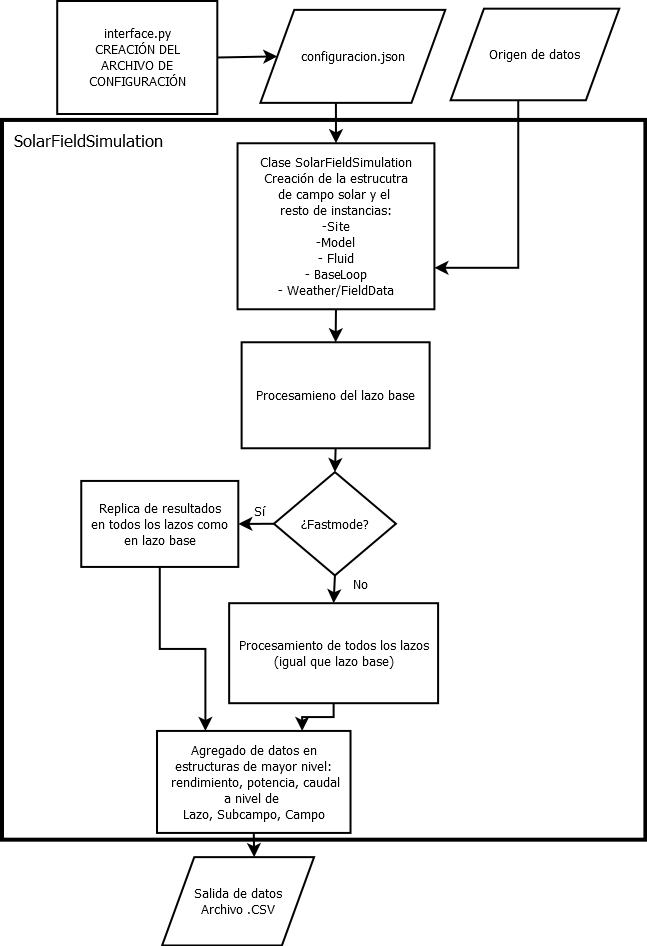
\includegraphics[width=0.80\linewidth]{images/flujo1.png}
\caption{Esquema de operación global de una simulación de un campo solar mediante la clase \texttt{SolarFieldSimulation}} 
\label{fig:flujo1}
\end{figure}

Según el tipo de simulación, durante el procesamiento del lazo se sigue o no un proceso de ajuste de caudal para conseguir obtener a la salida del lazo una temperatura determinada. El diagrama de flujo desarrollado para este bloque puede verse en la Fig.\ref{fig:flujo2}. En una misma ejecución del programa pueden ejecutarse ambas o solo una de las simulaciones.

\begin{figure}[H]
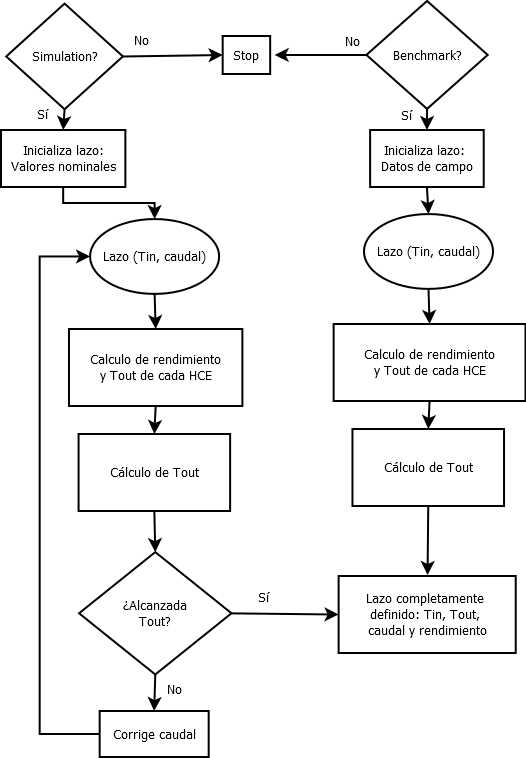
\includegraphics[width=0.80\linewidth]{images/flujo2.png}
\caption{Esquema desarrollado del bloque  de \emph{procesamiento del lazo} para las simulaciones tipo \emph{simulation} y \emph{benchmark}} 
\label{fig:flujo2}
\end{figure}

\section{Verificación por comparación con otra herramienta de simulación}

Con el fin realizar una primera verificación de nuestro código, compararemos en primer lugar los valores obtenidos para una determinada configuración de campo con los que se obtienen mediante System Advisor Model (SAM, \cite{freemanSystemAdvisorModel2018}), un software de reconocido prestigio muy empleado en el sector de las energías renovables. Las posibilidades de SAM van mucho más allá del alcance de nuestro código, pudiendo realizar el modelado no solo de sistemas de energía solar de concentración sino también de sistemas fotovoltaicos, geotérmicos, mareomotrices, eólicos, de biomasa por ejemplo. Dentro de los sistemas de energía solar térmica de concentración, ofrece la posibilidad de modelar centrales de las cuatro principales tecnologías ya comentadas y, a su vez, de diversas variedades dentro de cada una de éstas. SAM realiza también el análisis económico y financiero del proyecto basándose principalmente en la generación de electricidad que se espera producir. Por este motivo, SAM tiene en cuenta el acoplamiento del campo solar con el bloque de potencia a la hora de realizar la simulación.  Esto hace que no podamos comparar directamente nuestro programa con los modelos de SAM para generación eléctrica, pues los ajustes que hace SAM afectan al comportamiento del campo, introduciendo limitaciones de caudal de HTF y de potencia térmica transferida al bloque de potencia, desenfoques en el campo, rampas de arranque e inercias del sistema que quedan fuera de nuestro alcance. En cambio, SAM también cuenta con un módulo para la simulación de un sistema de generación de calor  para proceso industrial (IPH, Industrial Process Heat) basado en el modelo Físico que emplea para la simulación de plantas CCP. Emplearemos este módulo para comparar los resultados de SAM con nuestro simulador tal y como ese explica a continuación.

\subsection{Configuración de la simulación para comparación con SAM}
\label{configuracion-simulaciones}

Para que una simulación realizada con el módulo IPH de SAM sea comparable a la nuestra, indicaremos a SAM que no existe almacenamiento térmico para evitar los procesos de mezcla de HTF a diferentes temperaturas que se producirían en ese caso. También indicaremos que el sumidero térmico tiene capacidad elevada, lo que, en principio, nos obligaría a seleccionar un tamaño de campo solar muy grande. Para que el tamaño de campo solar sea igual al del campo que queremos simular indicaremos a SAM que las condiciones de radiación solar nominales son mucho más elevadas que las que se alcanzarán en cualquier momento el año (hemos puesto un valor de $(2000 W/m^2)$). De este modo, conseguimos que el dimensionado que hace SAM del campo solar sea igual que el nuestro (120 lazos), pero que a la largo de la simulación con datos de radiación reales no se produzca desenfoque en ningún momento. Es decir, con esta configuración de SAM extraemos del campo solar toda energía posible, al igual que hace nuestro simulador.

Puesto que solo modelamos el campo, no tenemos a priori ninguna información sobre la temperatura de retorno del HTF frío desde el intercambiador donde cede su energía al sumidero térmico. Con el fin de que la comparación sea lo más ajustada posible, aprovecharemos los datos de temperatura de HTF frío que se obtienen de la simulación de SAM como datos de entrada para nuestra simulación. De esta forma, en ambas simulaciones el salto térmico se realiza desde el mismo punto de partida. Además, indicaremos a SAM que no existe inercia térmica en tuberías y concentradores y prescindiremos del cálculo de pérdidas térmicas en las primeras.

Respecto al fluido caloportador, SAM nos permite seleccionar entre una serie de fluidos preconfigurados. Seleccionaremos \emph{Therminol VP-1} pues también podemos simular este fluido con nuestro programa.

Realizaremos la simulación para un año completo. Contamos con los datos meteorológicos del año 2007 en formato TMY3.  En la Fig.\ref{fig:captura01} se puede ver la pestaña de configuración de SAM para seleccionar el origen de datos meteorológicos.

\begin{figure}[H]
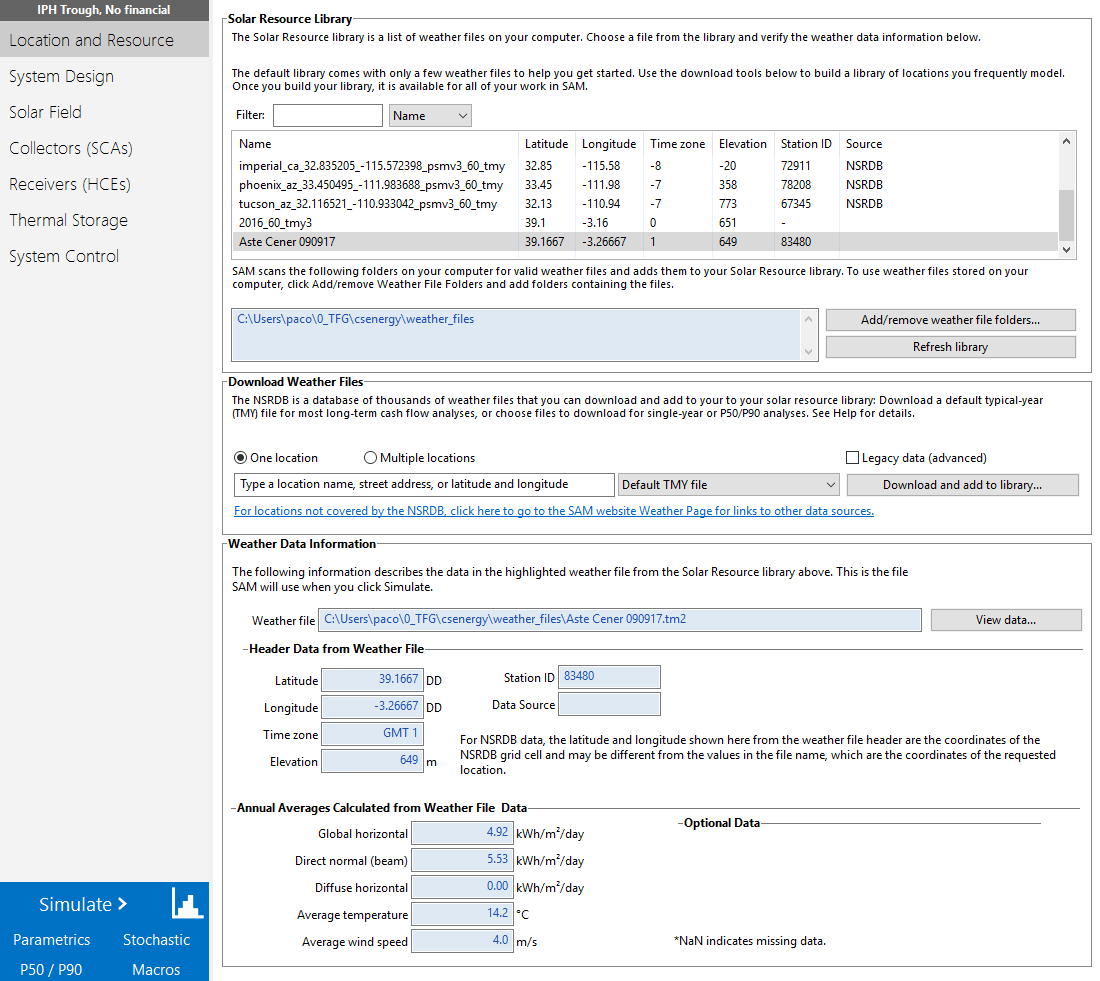
\includegraphics[width=0.9\linewidth]{images/captura_sam_iph01.png}
\caption{Configuración SAM. Seleccción del archivo de datos meterorológicos} 
\label{fig:captura01}
\end{figure}

La versión de SAM utilizada ha sido la \emph{''2020.2.29, 64 bit, updated to revision 1''}. En la Fig.\ref{fig:captura02} podemos ver la pestaña de configuración del campo solar. 

\begin{figure}[H]
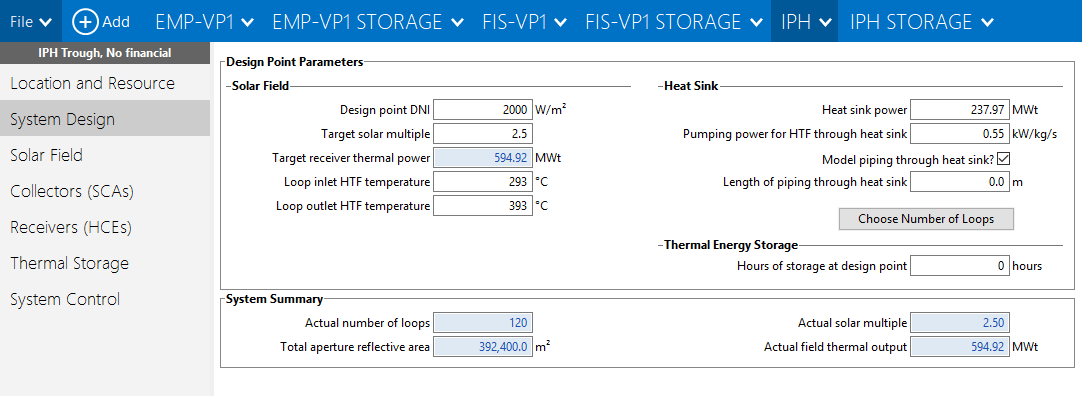
\includegraphics[width=0.9\linewidth]{images/captura_sam_iph02.png}
\caption{Configuración SAM. Campo solar} 
\label{fig:captura02}
\end{figure}

Los SCA, modelo SenerTrough I diseñado por Sener, se han parametrizado de la siguiente manera a partir del modelo EuroTrough ET150:

\begin{table}[H]
\centering
\caption{Configuración del SCA modelo SenerTrough I de Sener}
\label{tab:configuracionSCA}
\begin{tabular}{lc}
Parámetro & Valor \\ \hline
Longitud &  148,5  (m) \\
Apertura &  5,77  (m) \\
Distancia Focal & 2,1 (m) \\
Coeficiente $F_{0}$ del  IAM  &  1 \\
Coeficiente $F_{1}$ del  IAM  &  0,0506 \\
Coeficiente $F_{2}$ del  IAM  &  -0,1763 \\
Precisión del seguidor &  0,99 \\
Precisión geométrica &  0,98 \\
Disponibilidad &  0,99 \\
Reflectividad &  0,935 \\
Limpieza &  0,98
\end{tabular}
\end{table}


En la Fig.\ref{fig:captura03} puede verse una captura de pantalla de la pestaña de configuración del tipo de SCA en SAM. En la Fig.\ref{fig:captura04}, puede verse la pestaña correspondiente a la configuración de HCE. En este caso el modelo empleado es el UVAC 3, de Solel, con los parámetros que se indican en la tabla \ref{tab:configuracionHCE}.


\begin{figure}[H]
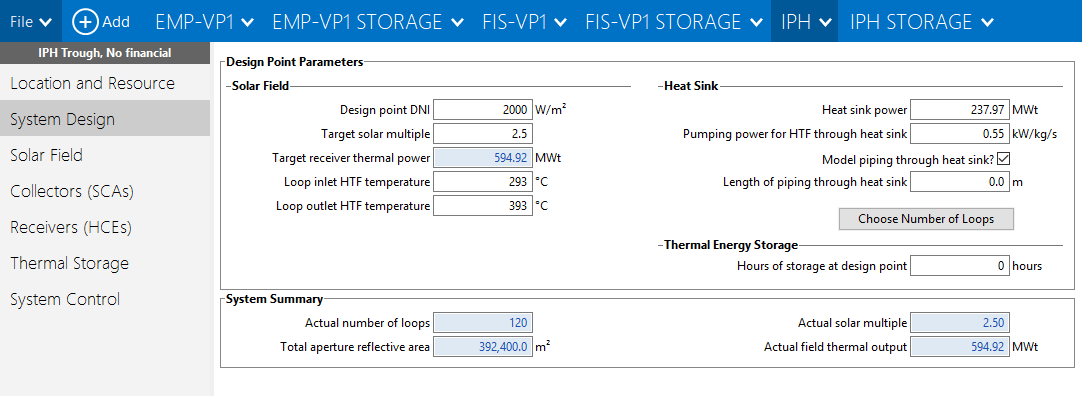
\includegraphics[width=0.9\linewidth]{images/captura_sam_iph02.png}
\caption{Configuración SAM. Configuración del SCA SenerTrough I a partir del modelo EuroTrough ET150} 
\label{fig:captura03}
\end{figure}

\begin{figure}[H]
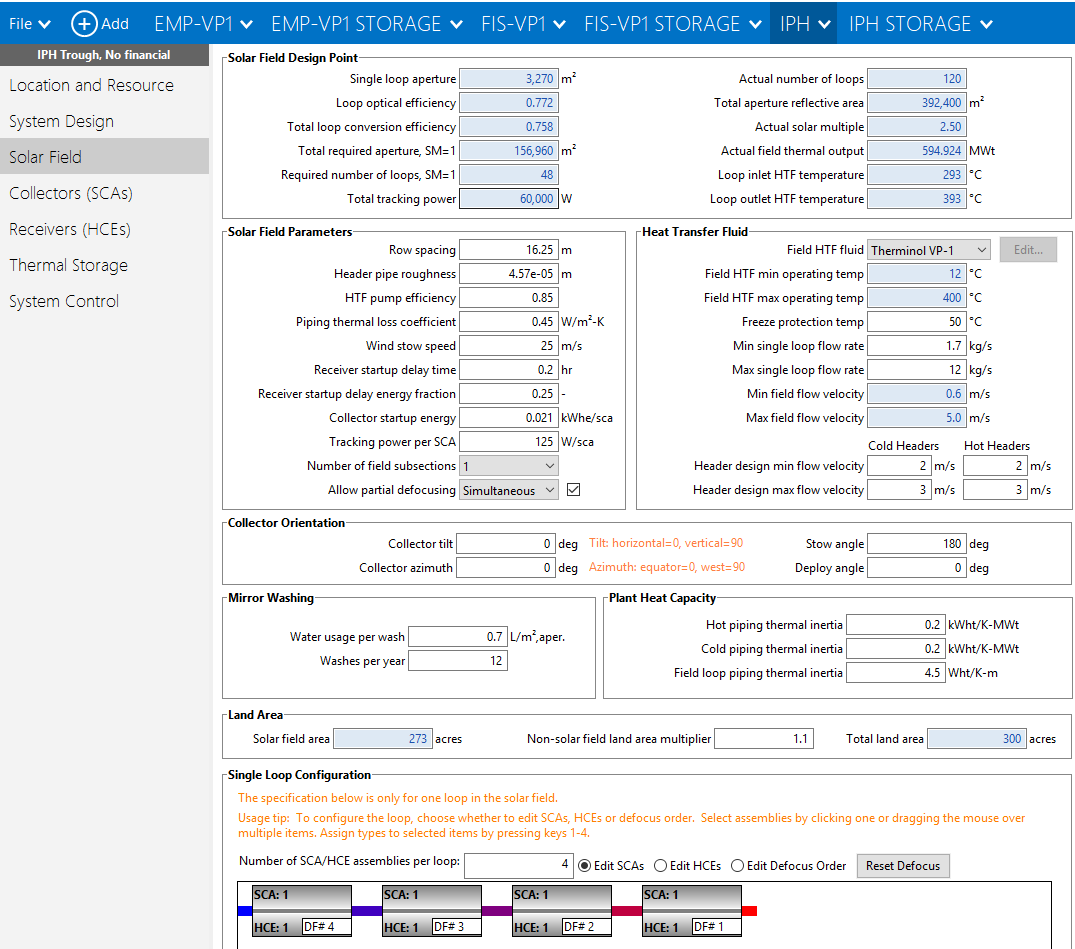
\includegraphics[width=0.9\linewidth]{images/captura_sam_iph03.png}
\caption{Configuración SAM. Configuración del HCE UVAC 3 con vacío}
\label{fig:captura04}
\end{figure}


\begin{table}[H]
\centering
\caption{Configuración del HCE modelo UVAC 3 de Solel}
\label{tab:configuracionHCE}
\begin{tabular}{lc}
Parámetro & Valor \\ \hline
Logintud & 4,05 (m) \\
Factor de longitud efectiva, \(\gamma_L\) &  0,96 \\
Factor de interceptación geométrica, \(\gamma_g\) & 0,96 \\
Diámetro interior del tubo absorbedor, \(D_{ri}\) & 0,066 (m) \\
Diámetro exterior del tubo absorbedor, \(D_{ro}\) &  0,070 (m) \\ 
Diámetro interior de la envolvente de vídrio, \(D_{gi}\) &  0,115 (m) \\
Diámetro exterior de la envolvente de vídrio, \(D_{go}\) &  0,121 (m) \\
Rugosidad interior &  0,000045 (m)  \\
Factor de emisividad, \(A_1\) &  0,000206 \\
Factor de emisividad, \(A_0\) &  0,0430 \\
Absortibidad solar del receptor &  0,96 \\
Transmisividad del vídrio &  0,96 \\
Valor mínimo del número de Reynolds recomendado &  2300 \\
Distancia de separación entre brazos de soportación &  4,05 (m) 
\end{tabular}
\end{table}

Se ha considerado que todos los HCE  del campo se encuentran en buen estado de vacío.

\subsection{Guía para la configuración de la simulación en Python}

Para la configuración de la simulación con nuestro código se debe crear un archivo en formato \emph{JSON} con el que se le pasa toda la información necesaria. Con el fin de facilitar la creación de este archivo de configuración se ha desarrollado una sencilla interfaz, \texttt{interface.py}, que sirve de guía durante el proceso. Aprovecharemos este apartado para crear la configuración al tiempo que nos sirve de breve guía de uso de la interafaz de usuario.

\subsubsection{Configuración de la simulación}
En la Fig.\ref{fig:interface01} se muestra la primera pantalla de la interfaz de configuración. Al abrir por primera vez se carga una plantilla con los datos de una configuración preestablecida. En la siguientes figuras se muestran los datos ya modificados según nuestras necesidades. El archivo de origen de datos que hemos seleccionado incluye los mismos datos meteorológicos que se han empleado para SAM y, además, los datos de temperatura de entrada del HTF al campo solar que ha generado SAM en la simulación IPH. También emplearemos el caudal calculado por SAM para compararlo con el que calcula nuestro simulador.

\begin{figure}[H]
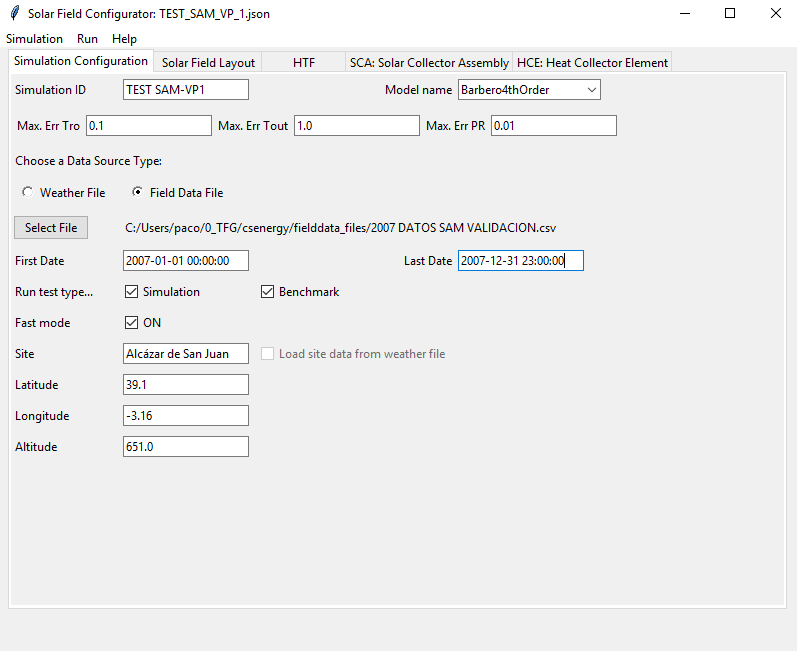
\includegraphics[width=0.9\linewidth]{images/interface01.png}
\caption[Configuración del tipo de simulación]{Configuración de la simulación. Selección del tipo de simulación, fichero de datos y lugar de emplazamiento.} 
\label{fig:interface01}
\end{figure}

En esta primera pestaña de la interfaz, el usuario puede dar un nombre identificador a la simulación. El campo \emph{Model name} es desplegable y permite seleccionar qué modelo se empleará para el cálculo del rendimiento térmico. Seguidamente, hay cuatro campos que permiten definir el máximo error permitido para la finalización del proceso iterativo:

\begin{itemize}
\item
\emph{Max. Err Tro} es el error absoluto en la temperatura de pared exterior, $T_{ro}$
\item
\emph{Max. Err Tout} es el error absoluto en la temperatura de salida del lazo, $T_{out}$
\item
\emph{Max. Err PR} es el error absoluto en el rendimiento térmico, $\eta$
\end{itemize}

De esta forma, el proceso iterativo continúa mientras los valores calculados entre dos iteraciones sucesivas presenten una diferencia superior a estos valores. Internamente se ha fijado un máximo de 1000 iteraciones, de tal forma que si no se alcanza convergencia tras ese número de ciclos el proceso muestra un mensaje y salta al siguiente punto.

Según se seleccione un origen de datos que incluya también datos de caudal y temperaturas de entrada y salida o, por el contrario, puramente meteorológico (\emph{Field Data File} o \emph{Weather File}), el programa nos permitirá, o no, realizar una simulación tipo \emph{benchmark}. 

La casilla de selección \emph{Fastmode} permite indicar que se realice la simulación considerando todos los lazos iguales o no. Esta opción es la única empleada en este trabajo pues, aunque es posible modificar a mano la estructura del campo solar para configurar cada lazo independientemente, en realidad está pensada para la inclusión en un futuro de un módulo que permita leer el estado de cada lazo en cada momento.

Si se selecciona la casilla \emph{Load site data from weather file}, la interfaz carga los datos del emplazamiento del fichero tipo \emph{Weather File} durante el proceso de carga. En caso contrario, los debe introducir el usuario.

\subsubsection{Configuración del Campo Solar}


En la Fig.\ref{fig:interface02} vemos cómo se configura el campo solar en un proceso similar al de SAM. Para esta simulación, con el fin acelerar el proceso de simulación, consideraremos que hay 2 HCEs en cada SCA. Es decir, cada HCE tiene una longitud de 72,9 m, que está por debajo del límite de 100 m que nos hemos impuesto como criterio de validez del tamaño de malla para el modelo unidimensional.  El caudal mínimo de recirculación en cada lazo es de 1,7 kg/s. La temperatura de salida deseada es de $393 ^\circ C$ (666,15 K).

\begin{figure}[H]
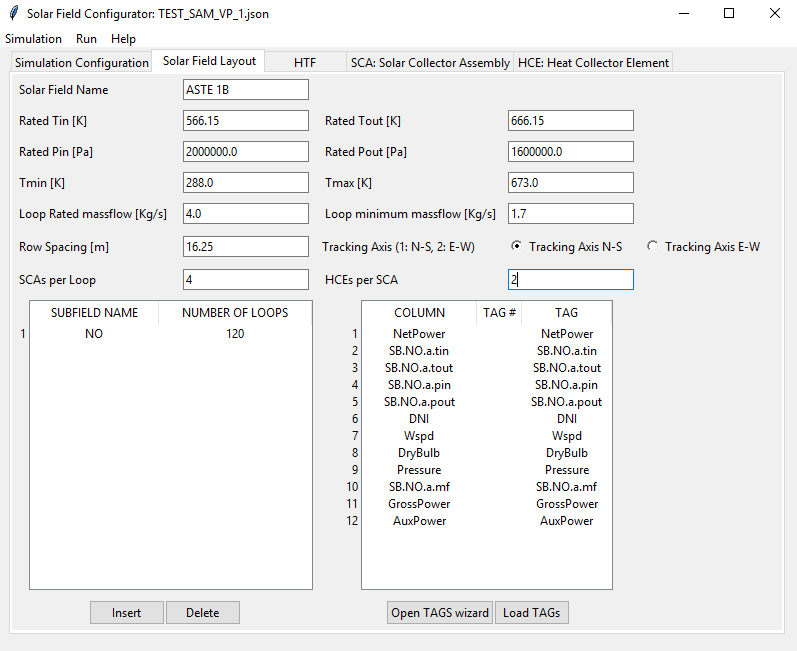
\includegraphics[width=0.9\linewidth]{images/interface02.png}
\caption[Configuración de la simulación del campo solar]{Configuración de la simulación. Configuración del campo solar, número de subcampos, lazos, configuración de los lazos, valores nominales y asistente para relacionar los identificadores de las columnas del archivo de origen de datos con los que maneja el programa.} 
\label{fig:interface02}
\end{figure}

Además de los valores nominales, que son empleados como punto de partida en las simulaciones, vemos que podemos configurar la orientación del eje del seguidor y el espaciado entre lazos para el cálculo de sombras. En la configuración de esta simulación hemos supuesto que existe un único subcampo con 120 lazos. La aplicación permitiría añadir varios subcampos mediante una lista de pares \emph{nombre de subcampo - número de lazos}. El nombre que se dé a los subcampos es relevante en el sentido de que, posteriormente, los archivos \emph{CSV} que se generarán  utilizarán una nomenclatura basada en esos nombres para mostrar las variables de temperatura, caudal, potencia, rendimiento, etc., de cada subcampo. 

En la Fig.\ref{fig:carga1} se muestra el proceso que permite establecer una relación entre los \emph{tags} o nombres que reciben los valores en el archivo de datos de campo y los valores que empleará el programa para el informe. El asistente muestra una lista (Fig.\ref{fig:listatags}) con los \emph{tags} disponibles junto a un número. El usuario debe indicar qué número corresponde a cada variable. Por ejemplo, el caudal másico del subcampo NO viene dado por el identificador número 10, \emph{1310-FX-1809}. Cuando ha terminado de asignar los números, debe pulsar \emph{Load TAGs} para que se cargue la lista, tal y como se ve en la Fig.\ref{fig:carga2}. Al quedar asociados de este modo, cuando el simulador cargue los datos del campo, sabe que debe emplear los datos de la columna con encabezado \emph{1310-FX-1809} como datos de caudal de ese subcampo.

\begin{figure}[H]
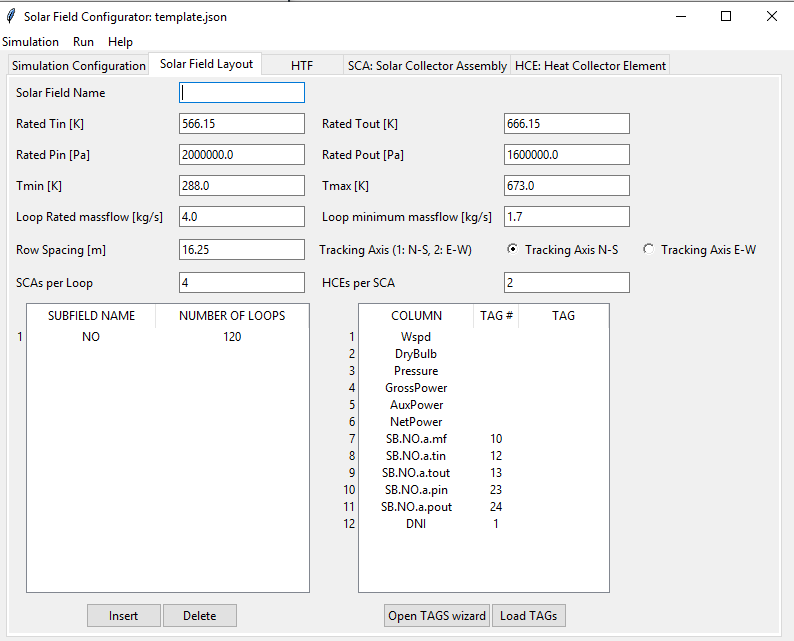
\includegraphics[width=0.9\textwidth, height=0.7\textwidth]{images/carga_tags.png}
\caption{Proceso de asignación de \emph{tags} a variables den entrada/salida}
\label{fig:carga1}
\end{figure}

\begin{figure}[H]
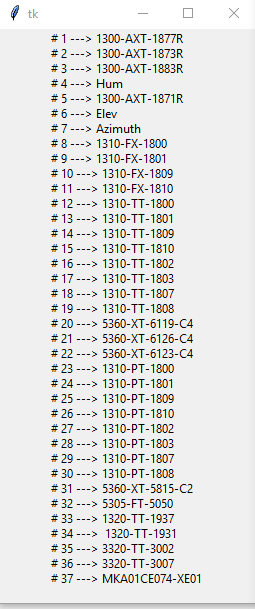
\includegraphics[width=0.3\textwidth, height=0.5\textwidth]{images/tagslist.png}
\caption{Ventana con la lista de \emph{tags} disponibles}
\label{fig:listatags}
\end{figure}

\begin{figure}[H]
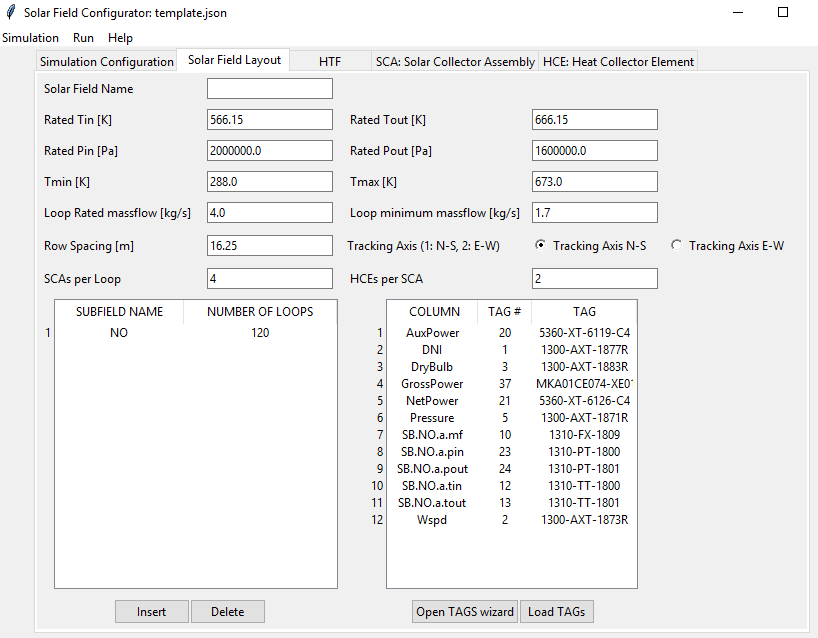
\includegraphics[width=0.9\textwidth, height=0.7\textwidth]{images/tagscargados.png}
\caption{Lista de asignaciones \emph{tag-variable} completa}
\label{fig:carga2}
\end{figure}

\subsubsection{Selección del fluido caloportador} 

El fluido caloportador \emph{Therminol VP-1} se configura tal y como puede verse en la Fig.\ref{fig:interface03}. El usuario puede optar por seleccionar los fluidos disponibles en la librería \emph{CoolProp}, con lo que los valores máximos y mínimos de trabajo quedan fijados a los que establece dicha librería. Actualmente la interfaz permite la selección de dos fluidos desde esta librería: \emph{Termninol VP-1} y \emph{Syltherm 800}. Otra posibilidad es seleccionar alguno de los fluidos para los que se dispone de los coeficientes de los polinomios que definen sus propiedades. En este caso, el fichero con la lista de fluidos se denomina \emph{fluids\_lib.json} y se puede editar directamente para añadir nuevos coeficientes. Una vez el fichero se ha cargado, se selecciona en el campo desplegable el fluido que se desee y los coeficientes se cargan en la tabla donde también pueden editarse.

\begin{figure}[H]
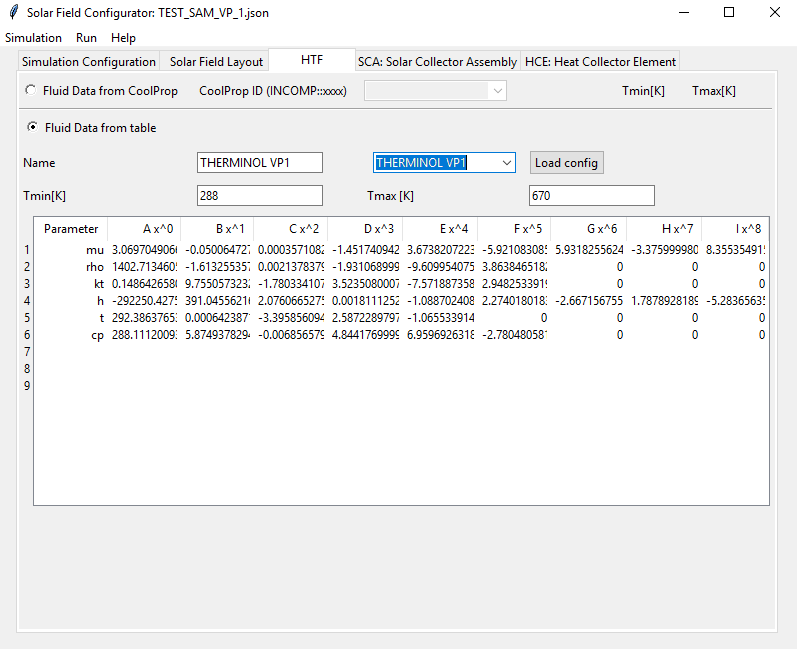
\includegraphics[width=0.9\linewidth]{images/interface03.png}
\caption{Configuración de la simulación. Selección y configuración del fluido caloportador} 
\label{fig:interface03}
\end{figure}

\subsubsection{Configuración del modelo de SCA} 

En la pestaña de configuración de SCA también disponemos de un campo desplegable en el que seleccionar algún modelo de SCA previamente almacenado en un fichero, en este caso denominado \emph{SCA\_lib.json}. De esta forma disponemos de los datos de distancia focal, los factores para el cálculo del IAM dados por el fabricante o la apertura. Todos los datos se pueden editar y modificar para realizar diversas pruebas, como variar las factores de limpieza, reflectividad, etc.

La pestaña de configuración de SCA con los datos correspondientes al modelo SenerTrough ya cargados puede verse en la Fig.\ref{fig:interface04}.

\begin{figure}[H]
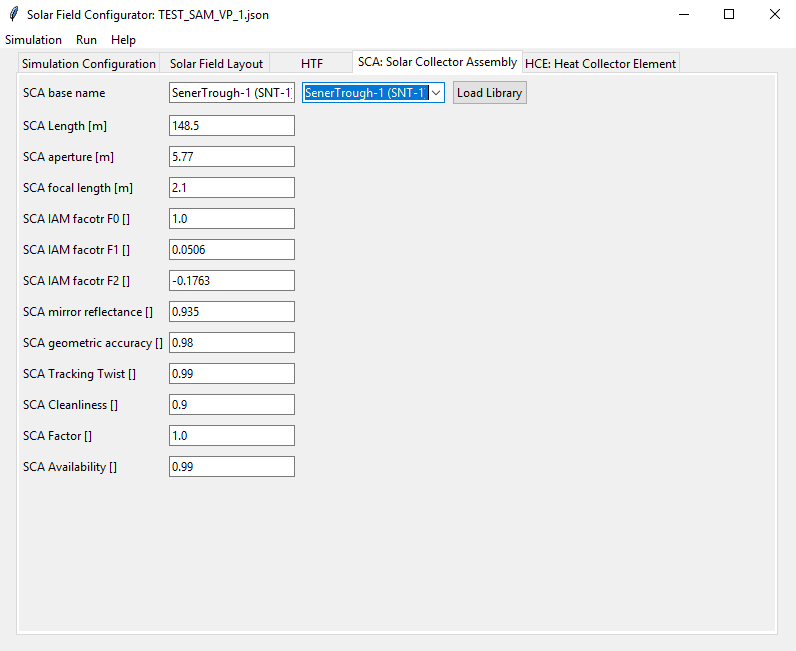
\includegraphics[width=0.9\linewidth]{images/interface04.png}
\caption{Configuración de la simulación. Selección del modelo de SCA y configuración} 
\label{fig:interface04}
\end{figure}


\subsubsection{Configuración del modelo de HCE} 
 
 Finalmente, en la Fig.\ref{fig:interface05} puede verse la configuración del modelo de HCE. Nuevamente disponemos de un archivo que almacena los datos de algunos modelos, denominado en este caso \emph{HCE\_lib.json}. Una vez seleccionado el  modelo que queremos, los datos se cargan y pueden ser editados. Es importante destacar que la longitud el HCE debe modificarse teniendo en cuenta el tamaño del SCA y e número de HCEs por SCA que hemos preconfigurado. Un pequeño texto nos da información sobre el numero máximo de HCEs que caben en el SCA según la longitud que indiquemos.

\begin{figure}[H]
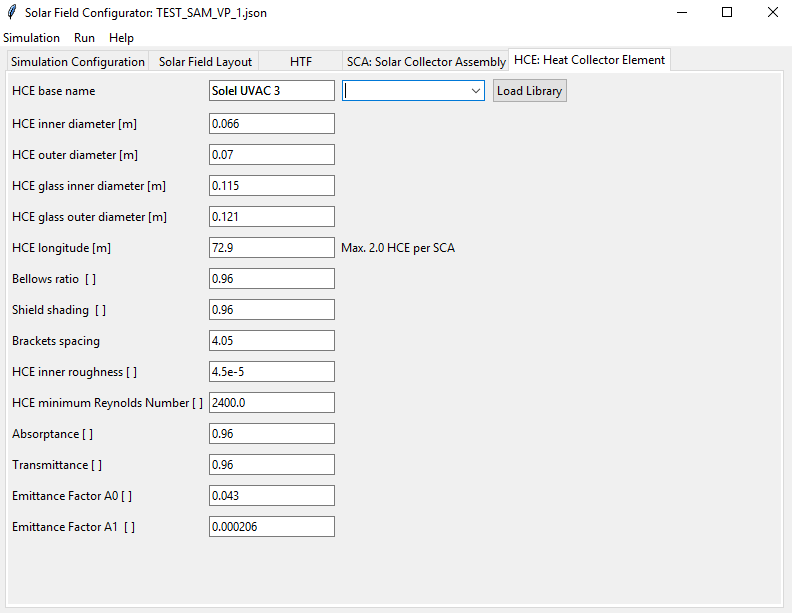
\includegraphics[width=0.9\linewidth]{images/interface05.png}
\caption{Configuración de la simulación. Selección del modelo de HCE y configuración} 
\label{fig:interface05}
\end{figure}


\subsubsection{Lanzamiento de la simulación}

Una vez hemos terminado de configurar nuestra simulación debemos guardarla con el nombre que queramos en un fichero. El resultado puede verse en el código \ref{lst:cfg}.  En este caso, los \emph{tags} coinciden con los nombres de las variables porque ya se habían modificado previamente   los encabezados de las columnas del archivo de origen de datos.

\begin{lstlisting}[caption=Fichero de configuración de la simulación en formato JSON, label={lst:cfg}]
{
 "simulation": {
  "ID": "TEST 2007 IPH",
  "datatype": 2,
  "simulation": true,
  "benchmark": true,
  "fastmode": true,
  "filename": "2007 IPH LOOP TEMP.csv",
  "filepath": "C:/Users/paco/0_TFG/csenergy/fielddata_files/",
  "first_date": "2007/01/31 00:00",
  "last_date": "2007/12/31 23:00"},
 "model": {
  "name": "Barbero4thOrder",
  "max_err_t": 0.1,
  "max_err_tro": 0.1,
  "max_err_pr": 0.01},
 "site": {
  "name": "Alcazar de San Juan",
  "latitude": 39.1,
  "longitude": -3.16,
  "altitude": 651.0},
 "loop": {
  "scas": 4,
  "hces": 2,
  "rated_tin": 566.15,
  "rated_tout": 666.15,
  "rated_pin": 2000000.0,
  "rated_pout": 1600000.0,
  "tmin": 288.0,
  "tmax": 673.0,
  "rated_massflow": 4.0,
  "min_massflow": 1.7,
  "row_spacing": 16.25,
  "Tracking Type": 1},
 "SCA": {
  "Name": "SenerTrough-1 (SNT-1)",
  "SCA Length": 148.5,
  "Aperture": 5.77,
  "Focal Len": 2.1,
  "IAM Coefficient F0": 1.0,
  "IAM Coefficient F1": 0.0506,
  "IAM Coefficient F2": -0.1763,
  "Track Twist": 0.99,
  "Geom.Accuracy": 0.98,
  "Reflectance": 0.935,
  "Cleanliness": 0.98,
  "Factor": 1.0,
  "Availability": 0.99},
 "HCE": {
  "Name": "Solel UVAC 3",
  "Length": 72.9,
  "Bellows ratio": 0.96,
  "Shield shading": 1.0,
  "Absorber tube inner diameter": 0.066,
  "Absorber tube outer diameter": 0.07,
  "Glass envelope inner diameter": 0.115,
  "Glass envelope outer diameter": 0.121,
  "Min Reynolds": 2400.0,
  "Inner surface roughness": 4.5e-05,
  "Envelope transmittance": 0.965,
  "Absorber emittance factor A0": 0.043,
  "Absorber emittance factor A1": 0.000206,
  "Absorber absorptance": 0.96,
  "Brackets": 4.05
 },
 "HTF": {
  "source": "table",
  "name": "THERMINOL VP1",
  "mu": [ 1.487, -0.02186, 0.0001400, -5.092e-07, 1.148e-09, -1.642e-12, 1.454e-15, -7.286e-19, 1.582e-22],
  "rho": [1403, -1.614, 0.002138, -1.931e-06, -9.610e-21, 3.864e-24, 0, 0, 0],
  "kt": [0.1486, 9.755e-06, -1.780e-07, 3.523e-12, -7.572e-25, 2.948e-28, 0, 0, 0],
  "h": [-292250, 391.0, 2.076, 0.001811, -1.089e-05, 2.274e-08, -2.667e-11, 1.788e-14, -5.284e-18],
  "t": [292.4, 0.0006424, -3.396e-10, 2.587e-16, -1.065e-22, 0, 0, 0, 0],
  "cp": [288.1, 5.875, -0.006857, 4.844e-06, 6.960e-20, -2.780e-23, 0, 0, 0],
  "tmax": 673.0,
  "tmin": 288.0},
 "subfields": [{"name": "NO", "loops": 120}],
 "tags": {
  "SB.NO.a.tin": "SB.NO.a.tin",
  "SB.NO.a.tout": "SB.NO.a.tout",
  "SB.NO.a.pin": "SB.NO.a.pin",
  "SB.NO.a.pout": "SB.NO.a.pout",
  "DNI": "DNI",
  "Wspd": "Wspd",
  "DryBulb": "DryBulb",
  "Pressure": "Pressure",
  "SB.NO.a.mf": "SB.NO.a.mf",
  "GrossPower": "GrossPower",
  "AuxPower": "AuxPower",
  "NetPower": "NetPower"
 }}
\end{lstlisting}
%\label{cfgsimulacion}
%\captionof{lstlisting}{Fichero de configuración de la simulación en formato JSON}
 
Desde la propia interfaz puede lanzarse la simulación mediante la opción de menú \emph{Run}, aunque también se puede lanzar la ejecución mediante un \emph{script} como el que se muestra en el código \ref{lst:script}, gracias a que se ha creado la Clase \texttt{SolarFieldSimulation} que se encarga de recibir el archivo de configuración y lanzar la simulación conforme a lo que en él se especifique.

\begin{lstlisting}[caption=Script para lanzar la simulación a partir del fichero JSON, label={lst:script}]
import json
import csenergy as cs
with open("./saved_configurations/TEST_2007_IPH_VP1.json") as simulation_file:
    SIMULATION_SETTINGS = json.load(simulation_file)
SIM = cs.SolarFieldSimulation(SIMULATION_SETTINGS)
SIM.runSimulation()
\end{lstlisting}

En la Fig.\ref{fig:ejecucion} vemos una captura de pantalla del inicio de la simulación en la consola de Python. Cuando el programa finaliza la ejecución, se guarda un fichero en formato \emph{CSV} con todos los datos calculados. El tamaño de este fichero puede ser de varios MB en el caso en que no se haya seleccionado la opción \emph{Fastmode}, ya que  de este modo se están almacenando, para cada fecha de cálculo, los datos de temperatura, caudal, potencia, y rendimiento de cada lazo, los agregados de los subcampos y el agregado del campo completo. Es decir, que puede tratarse de una tabla con varios cientos de columnas y, en caso de que la simulación sea para un año completo con datos horarios, de 8760 registros o filas.

\begin{figure}[H]
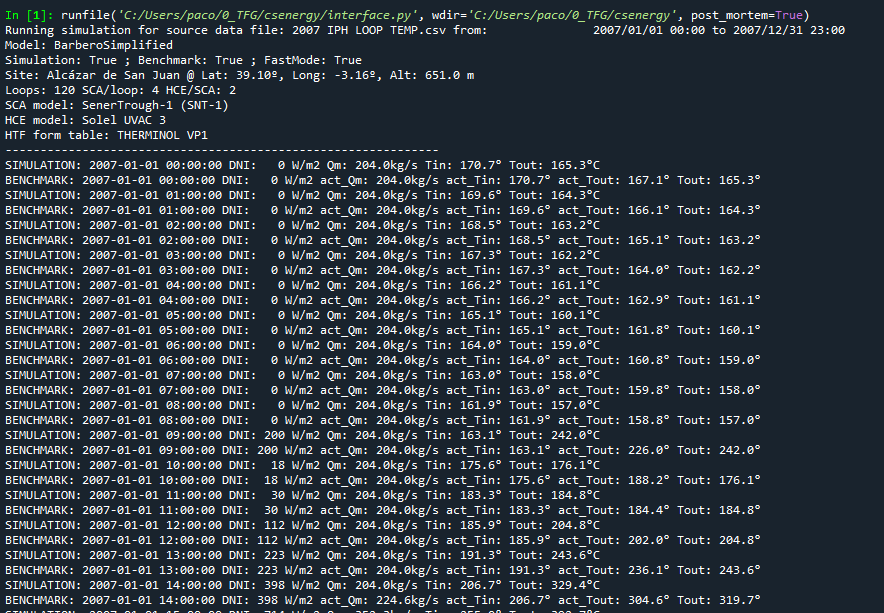
\includegraphics[width=0.9\linewidth]{images/ejecucion.png}
\caption{Consola de Python mostrando el inicio de una simulación} 
\label{fig:ejecucion}
\end{figure}

\subsubsection{Comentarios sobre los tiempos de ejecución}

El tiempo empleado para la simulación de un día completo (24 registros) de un campo de 120 lazos con 4 SCAs por lazo y 2 HCEs por SCA (es decir, HCE de unos 72 m), con la opción \emph{Fastmode} (todos los lazos idénticos) y en la que se ejecuta tanto la simulación tipo \emph{simulation} como la \emph{benchmark}, ronda los 4,75 segundos en un ordenador portátil con procesador Intel Core i5, 8 GB de memoria RAM y Windows 10 como sistema operativo. No parece un valor muy elevado pero si tenemos en cuenta los 365 días de un año el tiempo de ejecución llega a los 20 minutos aproximadamente para el año completo, muy superior a los tiempos habituales de simulación que emplean otras herramientas, como SAM, por ejemplo. Si vamos a una malla la mitad de pequeña (4 HCEs por SCA) el tiempo se duplica.  

Según las pruebas realizadas, hemos podido comprobar que la convergencia se suele alcanzar al cabo de unas pocas iteraciones (menos de 10 normalmente), pero el número de veces que se debe realizar este cálculo es importante, especialmente cuando se trata de ajustar el caudal hasta conseguir que la temperatura de salida sea la deseada. Además, el trasiego de datos entre las estructuras que se han creado es importante dado que, como  hemos indicado previamente, se almacena bastante información sobre cada lazo. Consideramos que la optimización del código puede acometerse en un futuro, una vez que el código haya podido ser depurado en mayor profundidad.

Para otro tipo de simulaciones, como las que se explican en el apartado \ref{analisis-parametrico} relativo al análisis paramétrico, los tiempos de ejecución son despreciables al no trabajar con volúmenes de datos tan grandes.


\subsection{Resultados de la verificación}
\label{resultados-validacion}
 
Una vez que tenemos configurado SAM y nuestro programa de la misma manera ejecutamos SAM sobre un archivo con los datos meteorológicos de un año y en valores horarios, en concreto se trata de los datos del año 2007 que se emplearon para el estudio y anteproyecto de construcción de plantas reales emplazadas en el mismo lugar para el que hemos configurado la simulación.  

En el campo solar de 120 lazos, con una superfice total de captación de 392400 $m^2$ la energía anual incidente es de 792,1 GWh, que se ve reducida a 686,4 GWh debido a que el ángulo de incidencia es distinto de cero (efecto coseno).

En la Tabla \ref{tab:generacion_anual} se muestran los valores  calculados por SAM y los que obtenemos con nuestro código. SAM denonima ''Receiver thermal power incident'' a la radiación solar que finalmente alcanza al absorbedor, es decir, la radaciación solar incidente menos las pérdidas ópticas. Este valor es equivalente a lo que nosotros hemos venido denominando potencia absorbida, $\dot q''_{abs}$. 

\begin{table}[H]
\centering
\caption{Resultados globales anuales para las simulaciones con SAM y Python}
\label{tab:generacion_anual}
\begin{tabular}{lcc}
Valores anuales  & SAM & Código Python \\ \hline
Potencia incidente (GWh/año)	& 686		& 686			\\ 
Potencia absorbida (GWh/año)	& 477		& 491			\\ 
Rendimiento óptico 			& 0,695	 	& 0,716			\\ 
Pérdidas térmicas (GWh/año)	& 64		& 73			\\ 
Rendimiento térmico			& 0,866		& 0,851			\\ 
Potencia térmica (GWh/año) 	& 413		& 418	        	\\ 
\end{tabular}
\end{table}

Comprobamos que existe una ligera desviación en el rendimiento óptico anual (2,9\%) y en el rendimento térmico anual (1,9\%). El origen de esta desviación se encuentra en la dificultad de adaptar exactametne la configuracón de nuestra simulación a la de SAM pues no todos los parámetros son equivalentes en ambos casos. Por otro lado, por tratarse de valores anuales, existe una acumulación de pequeñas desviaciones que se producen entre ambas simulaciones, principalmente a primera y última hora del día  y durante jornadas de gran inestabilidad en la radiación. 

Nos fijaremos ahora en el comportamiento a lo largo de un día completo. Hemos seleccionado un día de gran estabilidad y buena radiación solar y otro día menos estable y con peores condiciones. En las figuras \ref{fig:177caudal}  a \ref{fig:177potencia} podemos ver la evolución del caudal, la temperatura y la potencia térmica en ambas simulaciones para el día 17 de julio (buenas condiciones de radiación y estabilidad). En las figuras \ref{fig:176caudal}  a \ref{fig:176potencia} podemos ver la evolución para el día 17 de junio, con peores condiciones tal y como se aprecia por los altibajos que presentan las curvas a lo largo del día. En todas las gráficas se ha representado DNI en el eje secundario.

\begin{figure}[H]
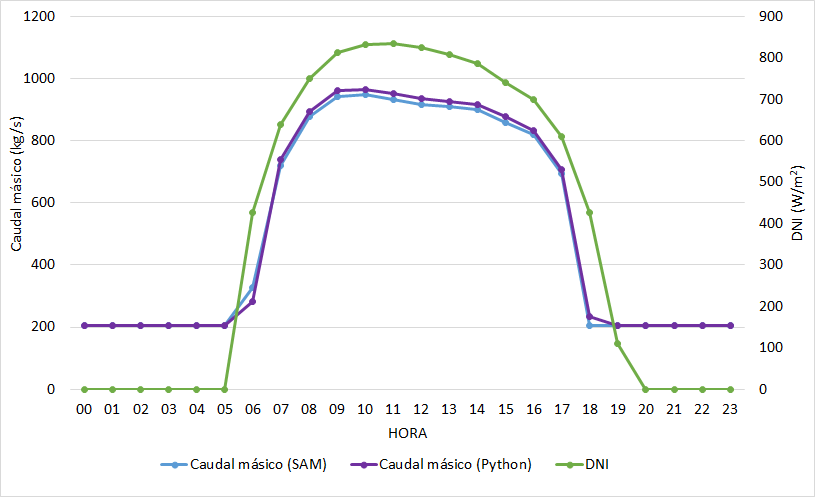
\includegraphics[width=0.9\linewidth]{images/177caudal.png}
\caption{Caudal másico calculado por SAM y por el código Python para el día 17/07/2007} 
\label{fig:177caudal}
\end{figure}

\begin{figure}[H]
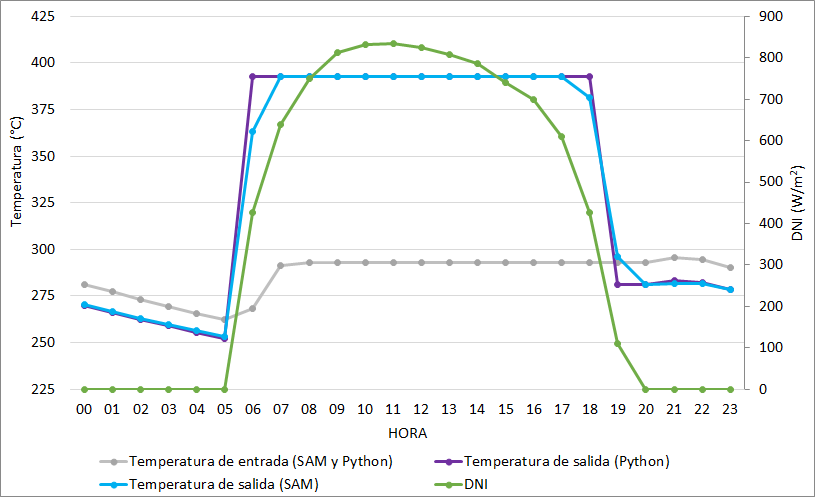
\includegraphics[width=0.9\linewidth]{images/177temperatura.png}
\caption{Temperatura de entrada y de salida calculadas por SAM y por el código Python para el día 17/07/2007} 
\label{fig:177temperatura}
\end{figure}

\begin{figure}[H]
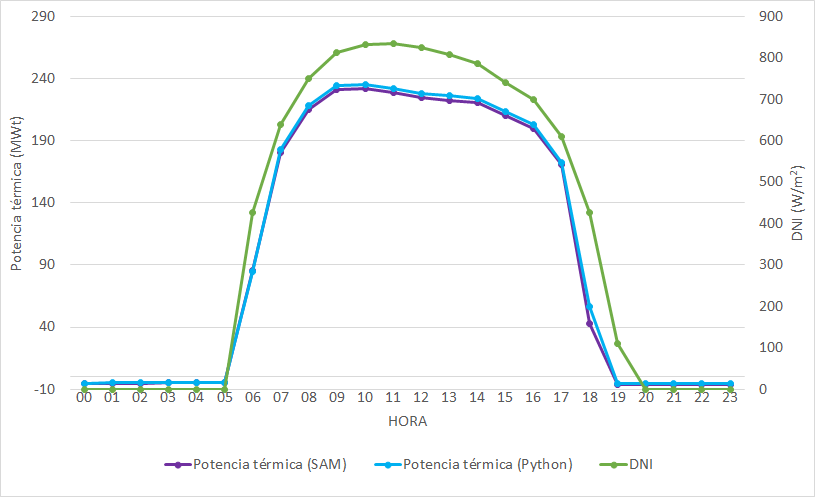
\includegraphics[width=0.9\linewidth]{images/177potencia.png}
\caption{Potencia térmica calculada por SAM y por el código Python para el día 17/07/2007} 
\label{fig:177potencia}
\end{figure}

La tabla \ref{tab:datos_17_julio} muestra los datos de caudal, temperatura y potencia para los 24 registros horarios del día 17 de julio.

\begin{table}[H]
\centering
\caption[Resultados de las simulaciones en un día de condiciones estables]{Resultados de las simulaciones (S: SAM, P: Python)  del día 17 de julio de 2007. Condiciones estables}
\label{tab:datos_17_julio}
\resizebox{\textwidth}{!}{%
\begin{tabular}{ccccccccc}
Hora &
\parbox{5em}{\centering DNI (S, P) \\ ($W/m^2$)} &
\parbox{5em}{\centering Caudal (S)  \\  ($kg/s$)}    &
\parbox{5em}{\centering Caudal (P)  \\  ($kg/s$)}  &
\parbox{5em}{\centering $T_{in}$ (S, P)  \\ $(^\circ C)$} &
\parbox{5em}{\centering $T_{out}$ (S)  \\ $(^\circ C)$} &
\parbox{5em}{\centering $T_{out}$ (P)  \\ $(^\circ C)$} &
\parbox{5em}{\centering Pot. Térmica (S)  \\  (MWt)}  &
\parbox{5em}{\centering Pot. Térmica (P) \\  (MWt)} \\ \hline
0:00  & 0   & 204,0 & 204,0 & 281,3 & 270,4 & 270,0 & -5,5  & -5,2  \\
1:00  & 0   & 204,0 & 204,0 & 277,2 & 266,6 & 266,2 & -5,3  & -5,0  \\
2:00  & 0   & 204,0 & 204,0 & 273,3 & 263,1 & 262,5 & -5,1  & -4,8  \\
3:00  & 0   & 204,0 & 204,0 & 269,5 & 259,6 & 259,0 & -4,9  & -4,7  \\
4:00  & 0   & 204,0 & 204,0 & 265,8 & 256,2 & 255,6 & -4,7  & -4,6  \\
5:00  & 0   & 204,0 & 204,0 & 262,3 & 253,0 & 252,3 & -4,6  & -4,4  \\
6:00  & 426 & 326,4 & 282,9 & 268,5 & 363,0 & 392,7 & 85,7  & 84,5  \\
7:00  & 639 & 721,1 & 739,0 & 291,4 & 392,6 & 392,9 & 180,1 & 182,8 \\
8:00  & 750 & 876,3 & 894,9 & 292,9 & 392,8 & 392,9 & 215,2 & 218,3 \\
9:00  & 812 & 943,4 & 961,0 & 293,0 & 392,5 & 392,9 & 230,7 & 234,3 \\
10:00 & 831 & 947,0 & 964,8 & 293,0 & 392,5 & 392,9 & 231,6 & 235,2 \\
11:00 & 834 & 933,5 & 951,8 & 293,0 & 392,6 & 392,9 & 228,4 & 232,0 \\
12:00 & 825 & 917,1 & 935,7 & 293,0 & 392,6 & 392,9 & 224,6 & 228,1 \\
13:00 & 809 & 908,3 & 926,8 & 293,0 & 392,7 & 392,9 & 222,6 & 225,9 \\
14:00 & 787 & 899,1 & 917,5 & 293,0 & 392,7 & 392,9 & 220,4 & 223,6 \\
15:00 & 740 & 857,7 & 876,1 & 293,0 & 392,9 & 392,9 & 210,6 & 213,5 \\
16:00 & 699 & 818,2 & 831,4 & 293,0 & 392,5 & 392,9 & 200,1 & 202,7 \\
17:00 & 610 & 694,2 & 706,8 & 293,0 & 392,9 & 392,9 & 170,5 & 172,3 \\
18:00 & 426 & 204,0 & 232,5 & 293,0 & 381,4 & 392,9 & 43,1  & 56,7  \\
19:00 & 109 & 204,0 & 204,0 & 293,0 & 295,9 & 281,0 & -6,4  & -5,6  \\
20:00 & 0   & 204,0 & 204,0 & 293,0 & 280,9 & 281,0 & -6,2  & -5,6  \\
21:00 & 0   & 204,0 & 204,0 & 295,7 & 281,4 & 283,5 & -6,3  & -5,7  \\
22:00 & 0   & 204,0 & 204,0 & 294,6 & 281,9 & 282,5 & -6,3  & -5,6  \\
23:00 & 0   & 204,0 & 204,0 & 290,5 & 278,6 & 278,6 & -6,0  & -5,5 
\end{tabular}%
}
\end{table}

\begin{figure}[H]
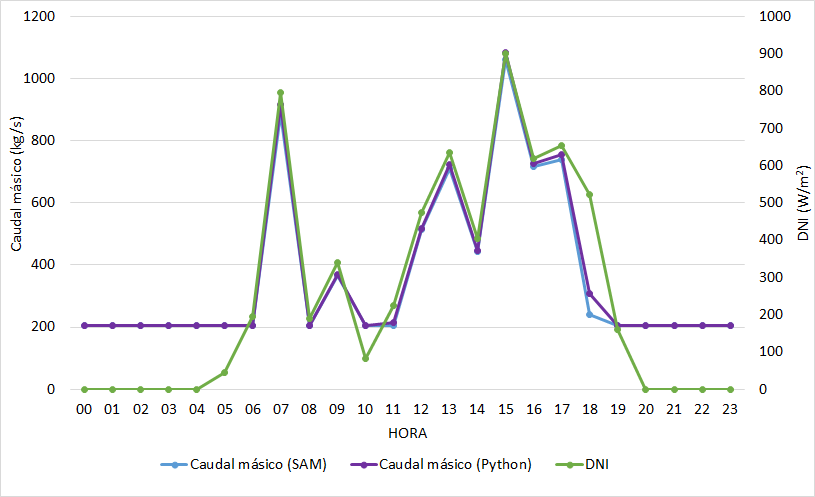
\includegraphics[width=0.9\linewidth]{images/176caudal.png}
\caption{Caudal másico calculado por SAM y por el código Python para el día 17/06/2007} 
\label{fig:176caudal}
\end{figure}

\begin{figure}[H]
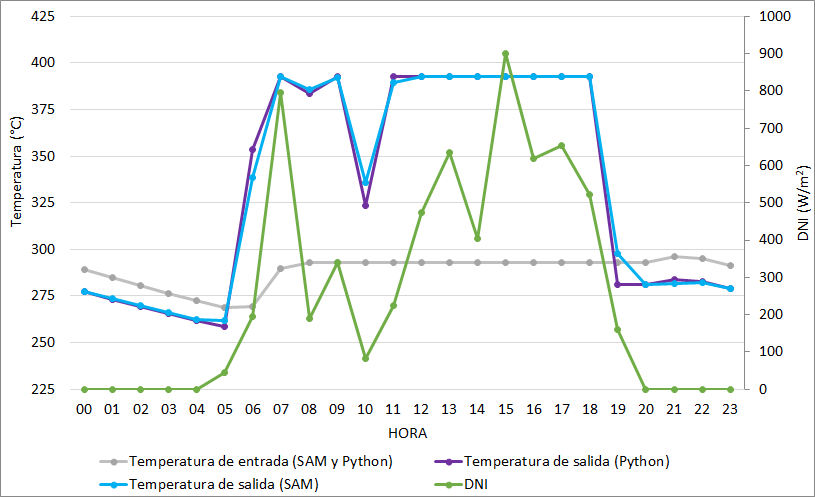
\includegraphics[width=0.9\linewidth]{images/176temperatura.png}
\caption{Temperatura de entrada y de salida calculadas por SAM y por el código Python para el día 17/06/2007} 
\label{fig:176temperatura}
\end{figure}

\begin{figure}[H]
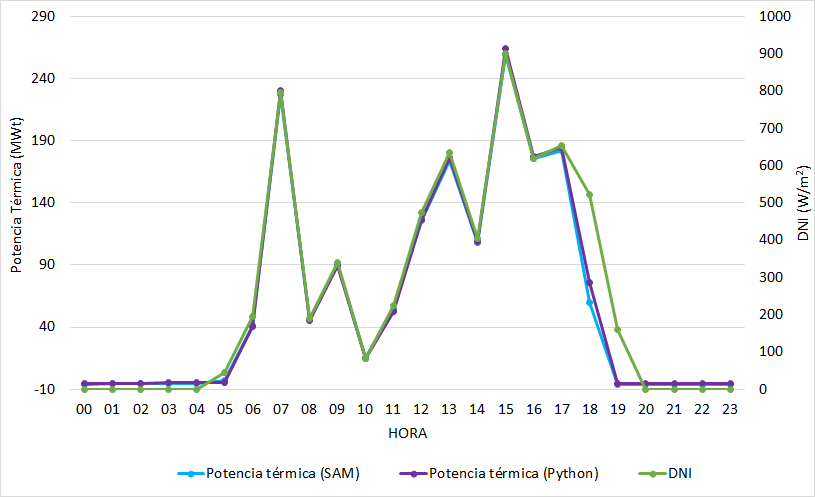
\includegraphics[width=0.9\linewidth]{images/176potencia.png}
\caption{Potencia térmica calculada por SAM y por el código Python para el día 17/06/2007} 
\label{fig:176potencia}
\end{figure}

En la tabla \ref{tab:datos_17_junio} se muestran los datos correspondientes al día 17 de junio de 2007.

\begin{table}[H]
\centering
\caption[Resultados de las simulaciones en un día de condiciones inestables]{Resultados de las simulaciones (S: SAM, P: Python) para el día 17 de junio de 2007. Condiciones inestables}
\label{tab:datos_17_junio}
\resizebox{\textwidth}{!}{%
\begin{tabular}{ccccccccc}
Hora &
\parbox{5em}{\centering DNI (S, P) \\ ($W/m^2$)} &
\parbox{5em}{\centering Caudal (S)  \\  ($kg/s$)}    &
\parbox{5em}{\centering Caudal (P)  \\  ($kg/s$)}  &
\parbox{5em}{\centering $T_{in}$ (S, P)  \\ $(^\circ C)$} &
\parbox{5em}{\centering $T_{out}$ (S)  \\ $(^\circ C)$} &
\parbox{5em}{\centering $T_{out}$ (P)  \\ $(^\circ C)$} &
\parbox{5em}{\centering Pot. Térmica (S)  \\  (MWt)}  &
\parbox{5em}{\centering Pot. Térmica (P) \\  (MWt)} \\ \hline
0:00  & 0   & 204,0  & 204,0  & 289,3 & 277,5 & 277,4 & -6,0  & -5,5  \\
1:00  & 0   & 204,0  & 204,0  & 284,8 & 273,5 & 273,3 & -5,8  & -5,3  \\
2:00  & 0   & 204,0  & 204,0  & 280,6 & 269,6 & 269,3 & -5,5  & -5,1  \\
3:00  & 0   & 204,0  & 204,0  & 276,5 & 265,9 & 265,5 & -5,3  & -5,0  \\
4:00  & 0   & 204,0  & 204,0  & 272,5 & 262,3 & 261,8 & -5,1  & -4,8  \\
5:00  & 45  & 204,0  & 204,0  & 268,8 & 262,0 & 258,4 & -3,2  & -4,7  \\
6:00  & 194 & 204,0  & 204,0  & 269,2 & 338,7 & 353,3 & 41,5  & 40,3  \\
7:00  & 795 & 885,8  & 916,9  & 289,7 & 392,7 & 392,9 & 227,1 & 230,5 \\
8:00  & 189 & 204,0  & 204,0  & 292,8 & 385,9 & 383,5 & 46,1  & 44,9  \\
9:00  & 339 & 366,8  & 367,7  & 292,9 & 392,2 & 392,9 & 90,0  & 89,7  \\
10:00 & 81  & 204,0  & 204,0  & 293,0 & 336,0 & 323,7 & 15,6  & 14,7  \\
11:00 & 225 & 204,0  & 215,4  & 293,0 & 389,6 & 392,9 & 53,8  & 52,5  \\
12:00 & 473 & 514,8  & 518,7  & 293,0 & 392,6 & 392,9 & 125,8 & 126,4 \\
13:00 & 634 & 711,7  & 722,5  & 293,0 & 392,5 & 392,9 & 174,1 & 176,1 \\
14:00 & 403 & 442,9  & 445,2  & 293,0 & 392,5 & 392,9 & 108,4 & 108,5 \\
15:00 & 899 & 1059,6 & 1082,5 & 293,0 & 392,7 & 392,9 & 259,6 & 263,9 \\
16:00 & 619 & 716,1  & 727,6  & 293,0 & 392,7 & 392,9 & 175,4 & 177,4 \\
17:00 & 654 & 740,2  & 755,1  & 293,0 & 393,0 & 392,9 & 181,9 & 184,1 \\
18:00 & 522 & 241,7  & 309,5  & 293,0 & 392,7 & 392,9 & 59,4  & 75,4  \\
19:00 & 160 & 204,0  & 204,0  & 293,0 & 297,8 & 280,9 & -6,5  & -5,6  \\
20:00 & 0   & 204,0  & 204,0  & 293,0 & 281,0 & 280,9 & -6,2  & -5,6  \\
21:00 & 0   & 204,0  & 204,0  & 296,2 & 281,6 & 283,8 & -6,4  & -5,7  \\
22:00 & 0   & 204,0  & 204,0  & 295,3 & 282,4 & 282,9 & -6,4  & -5,7  \\
23:00 & 0   & 204,0  & 204,0  & 291,1 & 279,1 & 279,1 & -6,1  & -5,6 
\end{tabular}%
}
\end{table}

En vista a los resultados de la comparación con SAM, consideramos que nuestro código obtiene valores adecuados y cuenta con la flexibilidad suficiente que permita emplearlo en la simulación del comportamiento de concentradores cilindroparabólicos. En el siguiente capítulo realizaremos algunos análisis a modo de ejemplo.


